\documentclass[11pt]{book} % use larger type; default would be 10pt

%%% PAGE DIMENSIONS
\usepackage{geometry} % to change the page dimensions
\geometry{a4paper, margin=1in} 
% or letterpaper (US) or a5paper or....
% change the margins to 2 inches all round
\usepackage{graphicx} % support the \includegraphics command and options
\usepackage[parfill]{parskip} % Activate to begin paragraphs with an empty line rather than an indent

%%% PACKAGES
\usepackage{booktabs} % for much better looking tables
\newcommand{\ra}[1]{\renewcommand{\arraystretch}{#1}} % More space between rows
% self-created command
\usepackage{natbib} % to use /citet command in citation
\usepackage{array} % for better arrays (eg matrices) in maths
\usepackage{paralist} % very flexible & customisable lists (eg. enumerate/itemize, etc.)
\usepackage{verbatim} % adds environment for commenting out blocks of text & for better verbatim
\usepackage{subcaption} % make it possible to include more than one captioned figure/table in a single float
\usepackage{cancel}
\usepackage{amsmath} % math symbols
\usepackage{amssymb} % math symbols
\usepackage[colorlinks = true, urlcolor=blue, linkcolor=blue, citecolor=black]{hyperref} % add url link in pdf
\usepackage[svgnames]{xcolor} % Required for colour specification
\usepackage{dirtree}
\usepackage{listings}
\newcommand{\plogo}{\fbox{$\mathcal{HY}$}} % Generic dummy publisher logo

\usepackage{color}
\usepackage{smartdiagram}
 
\definecolor{codegreen}{rgb}{0,0.6,0}
\definecolor{codegray}{rgb}{0.5,0.5,0.5}
\definecolor{codepurple}{rgb}{0.58,0,0.82}
\definecolor{backcolour}{rgb}{0.95,0.95,0.92}

\lstdefinestyle{mystyle}{
    backgroundcolor=\color{backcolour},   
    commentstyle=\color{codegreen},
    keywordstyle=\color{magenta},
    numberstyle=\tiny\color{codegray},
    stringstyle=\color{codepurple},
    basicstyle=\footnotesize,
    breakatwhitespace=false,         
    breaklines=true,                 
    captionpos=b,                    
    keepspaces=true,                 
    numbers=left,                    
    numbersep=5pt,                  
    showspaces=false,                
    showstringspaces=false,
    showtabs=false,                  
    tabsize=2
}

\lstset{style=mystyle}

%%% SECTION TITLE APPEARANCE
\usepackage{sectsty}   
\allsectionsfont{\sffamily\mdseries\upshape} 

%%% ToC (table of contents) APPEARANCE
\usepackage[nottoc,notlof,notlot]{tocbibind} % Put the bibliography in the ToC
\usepackage[titles,subfigure]{tocloft} % Alter the style of the Table of Contents
\renewcommand{\cftsecfont}{\rmfamily\mdseries\upshape}
\renewcommand{\cftsecpagefont}{\rmfamily\mdseries\upshape} % No bold!

%%% END Article customizations

\begin{document}

%----------------------------------------------------------------------------------------
%	TITLE PAGE
%----------------------------------------------------------------------------------------

\begin{titlepage} % Suppresses headers and footers on the title page
	
	\centering % Centre everything on the title page
	
	%------------------------------------------------
	%	Top rules
	%------------------------------------------------
	
	\rule{\textwidth}{1pt} % Thick horizontal rule
	
	\vspace{2pt}\vspace{-\baselineskip} % Whitespace between rules
	
	\rule{\textwidth}{0.4pt} % Thin horizontal rule
	
	\vspace{0.1\textheight} % Whitespace between the top rules and title
	
	%------------------------------------------------
	%	Title
	%------------------------------------------------
	
	\textcolor{Red}{ % Red font color
		{\Huge Coding}\\[0.5\baselineskip] % Title line 1
		{\Large IN}\\[0.5\baselineskip] % Title line 2
		{\Huge Fortran} % Title line 3
	}
	
	\vspace{0.025\textheight} % Whitespace between the title and short horizontal rule
	
	\rule{0.3\textwidth}{0.4pt} % Short horizontal rule under the title
	
	\vspace{0.1\textheight} % Whitespace between the thin horizontal rule and the author name
	
	%------------------------------------------------
	%	Author
	%------------------------------------------------
	
	{\Large \textsc{Hongyang Zhou}} % Author name
	
	\vfill % Whitespace between the author name and publisher
	
	%------------------------------------------------
	%	Time
	%------------------------------------------------
	
	{\large\textcolor{Red}{\plogo}}\\[0.5\baselineskip] % Publisher logo
	
	{\large\textsc{\today}} % Publisher
	
	\vspace{0.1\textheight} % Whitespace under the date
	
	%------------------------------------------------
	%	Bottom rules
	%------------------------------------------------
	
	\rule{\textwidth}{0.4pt} % Thin horizontal rule
	
	\vspace{2pt}\vspace{-\baselineskip} % Whitespace between rules
	
	\rule{\textwidth}{1pt} % Thick horizontal rule
	
\end{titlepage}

%----------------------------------------------------------------------------------------

\newpage
\tableofcontents
\newpage

%----------------------------------------------------------------------------------------
\chapter{Overview}

General reminder:
\begin{itemize}
\item The difference between theory and practice is less in theory than it is in practice.
\item Don't reinvent the wheel. Use reliable softwares and libraries, if possible.
\item Too many dependencies would kill your work.
\end{itemize}

%----------------------------
\section{Signature Features}

\verb|where| statement:
\begin{itemize}
\item arrays must have the same shape
\item code block can contain
\subitem Array assignments
\subitem other where constructs
\subitem forall constructs
\end{itemize}

Example: Stencil Update $A_{i}=0.5*(A_{i-1}+A_{i+1})$
\begin{lstlisting}[language=Fortran, caption=Stencil update 1D]
v(2:n-1) = 0.5 * (v(1:n-2) + v(3:n))
\end{lstlisting}
\begin{itemize}
\item Traditional scheme requires scalar variables
\item Array syntax: Evaluate RHS, then “copy” the result
\end{itemize}

Example: Stencil Update $A_{i,j}=0.25*(A_{i-1,j}+A_{i+1,j}+A_{i,j-1}+A_{i,j+1})$
\begin{lstlisting}[language=Fortran, caption=Stencil update 2D version 1]
a(2:n-1,2:n-1) = 0.25*(a(1:n-2,2:n) + a(3:n,2:n) + a(2:n,1:n-2) + a(2:n,3:n))
\end{lstlisting}
Or using forall statement:
\begin{lstlisting}[language=Fortran, caption=Stencil update 2D version 2]
forall (i=2:n-1, j=2:n-1) &
a(i,j) = 0.25*(a(i-1,j) + a(i+1,j) + a(i,j-1) + a(i,j+1))
\end{lstlisting}
\begin{itemize}
\item Fortran statement looks exactly like the original formula.
\end{itemize}

%----------------------------------
\section{What's Falling Behind}

\subsection{Preprocessor}

Conditional compilation has never really caught on in Fortran and there isn't a standard pre-processor.
This limits the usage of many features, e.g., assertion.

\subsection{MPI Standard Library}

Can you imagine that there are three officially supported MPI library in Fortran?
It is just because Fortran is old, and no one wants to touch the old code; so even if new features are added, like the argument checking in \verb|mpi_f08|, very few codes are actually using it.

\subsection{I/O}

The general trend is that it is becoming more and more C-like. After Fortran 2003, you can even find the concept of stream!

From the benchmark done on the \href{https://julialang.org/benchmarks/}{Julia Website}, Fortran is 6 times slower in terms of writing to file.

\subsection{Interfering with Command Line}

Can you imagine that a simple task like mkdir is not still not available in Fortran? Fortran compiler vendors now provide a general interface to the command line, \verb|execute_command_line|, to handle these kinds of problems.

\subsection{Coroutines}

It may once be a good attempt, but end in no where, because no one is actually using this built-in parallel feature.

%----------------------------------
\section{Variables}

There are several things you need to pay attention with regard to variables.

\subsection{Variable Scope}

Module variables have the intrinsic \verb|save| attribute, which means that they will be allocated only once and stay there until the end of your program. In some programming languages, it is equivalent to \verb|static|. A clear usage of \verb|use| statement helps you organizing the available scopes. It is nice to add \verb|ONLY| to limit your data scope.

Things get a little bit complicated with OpenMP included, but still, there are rules to follow.


\subsection{Allocations}

Local variables within functions are allocated on the stack (first in, first out), while dynamic variables are allocated on the heap.

Potential issues with variable allocation on the heap:
\begin{itemize}
\item The size of the stack is severely limited. (Check the specific default!)
\item Remedies are problematic (Intel: -mcmodel=medium -intel-shared)
\end{itemize}

\subsection{Garbage Collection}

Modern compilers all have automatic garbage collections, so in general we as programmers don't need to worry about deallocating arrays. Explicit deallocating user-defined large arrays that won't be used later on is always not bad. However, there are cases in which you don't want to deallocate intermediate arrays that will be used again in a loop. Mark them with \verb|save| and allocate them only once.


%--------------------------------
\section{Modules}

Modules stay in the key concept of Fortran90+. After Fortran 2008: Modules may contain Submodules.
Modules have to be compiled first, with each results in a \verb|.mod| file.

At linking time, the module is known through the \verb|.mod| file.

What to put in a Module:
\begin{enumerate}
\item Constants (parameters)
\item Derived type declarations
\subitem avoid repeating parameter and derived type definitions. Sometimes physical constants are put in an include file. This should be done using a module.
\item Global variables
\item Related functions and subroutines.
\subitem move on by using the public, private and protected attributes
\item Write Object-Oriented code without performance penalty
\item Use Inheritance and Polymorphism with care
\end{enumerate}


\subsection{Compiling Modules}

The module name need not be the file name; doing that is strongly recommended, though.

Now you compile it , but don't link it:
\begin{verbatim}
nagfor -C=all -c mymod.f90
\end{verbatim}
It will create files like \emph{mymod.mod} and \emph{mymod.o}. They contain the interface and the code. The interfaces are like compiled headers. You don’t do anything with these, explicitly: the compiler will do find them and use them.

To add another search path , use -I$<directory>$.

Compile all of the modules in a dependency order. If A contains USE B , compile B first. Then add a *.o for every module when linking:
\begin{verbatim}
nagfor -C=all -o main main.f90 mod_a.o mod_b.o mod_c.o
\end{verbatim}

\subsection{Use Statements}

Proposed syntax
\begin{verbatim}
USE [[, module-nature] ::] module-name [AS use-name] [, ONLY:only-list]
\end{verbatim}

Without “AS use-name” it is a regular USE statement. However, when the “AS use-name” is used, then the entities defined in module “module-name” are accessed only with “use-name\%entity-name” syntax.


%-----------------------------
\section{Miscellaneous}

Benefits:
\begin{itemize}
\item Allows consistency check by the compiler
\item Assume-shape arrays, optional parameters, etc.
\end{itemize}

intent: (in/out, inout) maintainability

optional

any, all

Using generic interfaces for functions

User-defined operators

Elemental function used with \emph{all} and \emph{where}: similar to bitwise operations in Matlab

Inquiry functions (see slides)

Pointers: useful for creating ``linked lists''; avoid copying data

Command line arguments

get environment variable inside Fortran (e.g. home directory)

Pure function is used to prevent any input arguments being modified, regardless of the use of \verb|intent| statement.

Elemental function is used to create procedures that operate parameters of arbitrary dimension.


%-------------------------------------------------------
\section{Naming Standard}
\begin{quote}
There are only two hard things in Computer Science: cache invalidation and naming things. --- Phil Karlton
\end{quote}

Good variable names are crucial, especially in dynamically typed languages, where you don't have types defined to help you make sense of the variables. However, even statically typed languages will have the benefit of better readability when good naming conventions are used.

\subsection{Arrays}

Arrays are an iterable list of items, usually of the same type. Since they will hold multiple values, pluralizing the variable name makes sense.

\begin{lstlisting}[language=java, caption=Array names]
// bad
const fruit = [`apple', `banana', `cucumber'];
// okay
const fruitArr = [`apple', `banana', `cucumber'];
// good
const fruits =  [`apple', `banana', `cucumber'];
// great
const fruitNames =  [`apple', `banana', `cucumber'];
// great
const fruits = [{
   name: `apple',
   genus: `malus'
}, {
   name: `banana',
   genus: `musa'
}, {
   name: `cucumber',
   genus: `cucumis'   
}];
\end{lstlisting}

\subsection{Booleans}

Booleans can hold only 2 values, \verb|true| or \verb|false|. Given this, using prefixes like ``is'', ``has'' and ``can'' will help the reader infer the type of the variable.

\begin{lstlisting}[language=java, caption=Booleans names]
// bad
const open = true;
const write = true;
const fruit = true;

// good
const isOpen = true;
const canWrite = true;
const hasFruit = true;
\end{lstlisting}

What about predicate functions (functions that return booleans)? It can be tricky to name the value, after naming the function. Usualy prefix with either \verb|check| or \verb|get| would be nice.

\subsection{Numbers}

For numbers, think about words that describe numbers.

\subsection{Functions}

Functions should be named using a verb, and a noun. When functions perform some type of action on a resource, its name should reflect that. For example, \verb|getUser|, \verb|toUppercase|.

Another common naming pattern is when iterating over items. When receiving the argument inside the function, use the singular version of the array name:
\begin{lstlisting}[language=java, caption=Iterating over items]
const newFruits = fruits.map(fruit => {return doSomething(fruit)});
\end{lstlisting}

\subsection{Blocks}

Block works like a local scope, similar to brackets in C/C++. You can define local variables that won't interfere with others.

\subsection{Summing up}
Take these naming convections with a pinch of salt. How you name your variables is less important than naming them consistently.

%-------------------------------------------------------
\section{Interoperatability}

\subsection{Mixture with C}
A Fortran90+ program, subroutine, or function that will call a C function might try using the ISO C binding module. This was actually introduced as part of Fortran 2003, but your compiler may be willing to let your Fortran90 program access it. (If not, you might consider moving to Fortran 2003!). 

The ISO C bindings are made available by the statement:
\begin{verbatim}
use iso_c_binding
\end{verbatim}

You can also use fussier versions of this statement, such as
\begin{verbatim}
use, intrinsic :: iso_c_binding
\end{verbatim}
or
\begin{verbatim}
use, intrinsic :: iso_c_binding, only : C_CHAR, C_NULL_CHAR
\end{verbatim}

Once you have the C bindings, you need to define an interface to your C function, which might read:
\begin{lstlisting}[language=Fortran, caption=C interface]
interface
    subroutine kronrod ( n, eps, x, w1, w2 ) bind ( c )
      use iso_c_binding
      integer ( c_int ), VALUE :: n
      real ( c_double ), VALUE :: eps
      real ( c_double ) :: x(*)
      real ( c_double ) :: w1(*)
      real ( c_double ) :: w2(*)
    end subroutine kronrod
end interface
\end{lstlisting}

Finally, to guarantee that FORTRAN and C agree on data types, you should declare any Fortran90 variables that will be passed through the C interface with statements like this, which essentially specify the appropriate KIND parameter to guarantee compatibility:
\begin{lstlisting}[language=Fortran, caption=C interface]
  integer ( c_int ), parameter :: n = 3
  real ( c_double ) eps
  real ( c_double ) x(n+1)
  real ( c_double ) w1(n+1)
  real ( c_double ) w2(n+1)
\end{lstlisting}

Note:
\begin{enumerate}
\item If you use subroutines in Fortran, set the return value of C functions to void, and use pointers because Fortran always passes by reference.
\item If you use functions in Fortran, set the return value as it is.
\end{enumerate}

\subsection{Mixture with C++}
Much similar to C, except a special requirement when C++ is involved is that the extern "C" qualifier be used with all the function names that must be "visible" to the Fortran90 program. For this example, we simple declare all the C++ functions this way:
\begin{verbatim}
extern "C" {
  long long f_(long long *a, long long *b, long long *c, long long *d);
  void ftest_(int *a, int *b);
}
\end{verbatim}

\subsection{Mixture with CUDA}

See this \href{https://stackoverflow.com/questions/35150748/mixed-language-cuda-programming}{demo}.


\section{Code Development}
using FORD (FORtran Documenter) to build html:
\href{https://github.com/Fortran-FOSS-Programmers/ford}{FORD}

I need to look deeper into this app for a better understanding of the structure of BATSRUS. It will also be useful for a diagram showing the structure of a complex code. Ford is written in Python and is target specifically at Fortran.

Graphviz can be used to generate graph descriptions of the program.

%------------------------
\section{Attribute}

A variable with the SAVE attribute retains its value and definition, association, and allocation status on exit from a procedure. All variables accessible to a main program are saved implicitly. 

A local variable that is initialized when declared has an implicit SAVE attribute. Explicit initialization of a module variable that is not in a common block implies the SAVE attribute.

Variables don't need to be deallocated by the programmer. The garbage collection technique handles this.

When intent(out) is used with a derived type, any component not assigned in a procedure could become undefined on exit. For example, even though a\%y was defined on entry to this routine, it could become undefined on exit because it was never assigned within the routine.

As an alternative, use intent(inout) to avoid the issue.


%-----------------------
\section{Pointer}

Does pointer affect performance? I have a simple test program for showing the differences between using pointers, stack allocated arrays, and heap allocated arrays. The results show that:
\begin{table}[]
\begin{tabular}{lllll}
\hline
Optimization & stack array & pointer & heap array & no small array\\
\hline
-O0          & 0.998 s       & 1.829 s  & 1.120 s  & 1.045 s   \\
-O2          & 0.928 s       & 1.519 s   & 0.940 s  & 0.884 s \\
-O3          & 0.886 s      & 0.853 s   & 0.884 s  & 0.839 s  \\
-Ofast       & 0.890 s       & 0.868 s  & 0.889 s & 0.848 s\\
\hline
\end{tabular}
\end{table}

With higher level of optimization, pointer performs better than local copies!


%-----------------------
\section{Debug}

I once encountered a very strange bug in a serial Fortran 77 code. It behaved like a local unused variable will cause the program to give different output.

%-----------------------
\chapter{Object Oriented Programming}

\section{Introduction}

OOP on access control

OOP may be slower (if not written carefully)

You can organize your data by defining your own structures and derived types. A good usage of user defined objects will simplify your program a lot.
As poor Fortran people we are used to simply translate formula, we do not care about paradigms… What Paradigm is the following?

\begin{lstlisting}[language=Fortran, caption=Procedural programming style]
subroutine solr(toll,Qm,gamma1,a1,u1,p1,rho1,gamma4,a4,u4,p4,rho4,u,p,a,fF)
  real*8 a2,p2,rho2,a3,p3,rho3,ps,us
  real*8 pn,pn_1
  real*8 a,u,p
  real*8 w1,w4,toll,Qm
  real*8 delta,gamma,gm1
  ...
  gm1=gamma-1.d0
  delta=gm1/2.d0
  alfa=(p1/p4)**(gm1/(2.d0*gamma))
  beta=alfa*delta/a1+delta/a4
  ...
\end{lstlisting}

Aside from being very ugly, the above example shows that data is \textbf{highly decoupled}. This is typical of \textbf{procedural programming} paradigm:
\begin{itemize}
\item TOP to down approach
\item focus on the operations, not on the data
\item data handling unsafe, GLOBALS are often necessary
\item hard to add new functionality or change the work flow without going back and modifying all other parts of the program
\item not easily reusable, so programmers must often recreate the wheel
\item difficult to maintain
\end{itemize}

Change your point of view!
\begin{itemize}
\item down to TOP approach
\item key idea: \emph{The real world can be accurately described as a collection of \textbf{objects} that interact}
\end{itemize}

How-To-OOP, the Pillars
\begin{itemize}
\item Encapsulation;
\item Inheritance;
\item Polymorphism.
\end{itemize}

\subsection{Encapsulation}
Encapsulation is about grouping of functionality (methods) and related data (members) together into a coherent data structure, \textbf{classes}.

\textbf{Implementation} is hidden from the rest of the program, aka Application Program Interface.

Do you need to know exactly how every aspect of a car works (engine, carburettor, alternator…)? No --- you only need to know how to use the steering wheel, brakes, accelerator…

In practice,
\begin{itemize}
\item restrict access to data (and data hiding):
\item more control;
\item easy to debug;
\item easy to maintain;
\item avoid side effects;
\item easy to parallel.
\end{itemize}

The Consequences:
\begin{itemize}
\item design by-contract
\item modularize;
\item abstraction;
\item develop by tests.
\end{itemize}

\underline{Example}: gas\_t

So, where is encapsulation? The user of \textbf{gas} class is not aware of how to compute the speed of sound. He/she simply uses the speed of sound; cannot manipulate gas data directly…
a bad user cannot make density negative manually;
can re-use the same names defined into \textbf{gas\_t} module:
encapsulation allow easy handling of names-collision (safety names space).

\subsection{Inheritance}
Inheritance enables new objects to take on the properties of existing objects, the \textbf{base class}. A child inherits visible properties and methods from its parent while adding additional properties and methods of its own.

In practice,
\begin{itemize}
\item re-use existing classes:
\item reduce code-duplication:
\item easy debug;
\item easy maintain;
\item inherit members/methods;
\item re-use implementation;
\item classes hierarchy;
\item abstract is better, but specials happen…
\item specialize only when/where is necessary.
\end{itemize}

The Consequence
\begin{itemize}
\item design from down to up…
\item from very down! Abstract all!
\item specialize $\Rightarrow$ inherit from abstract to concrete cases
\item avoid to re-invent the wheel
\end{itemize}

So, where is inheritance? The development of \textbf{multifluid gas} class. We do not need to re-implement all the behaviors of gas class: multifluid is a special gas… avoid-re-invent the wheel;
While the user of \textbf{multifluid gas} class found the same facility of the previous gas class:
avoid to re-learn from scratch;
could re-use his/her own applications designed for gas objects…

\subsection{Polymorphism}
Polymorphism is the concept that multiple types of objects might be able to work in a given situation.
If you needed to write a message on a piece of paper, you could use a pen, pencil, marker or even a crayon. You only require that the item you use can fit in your hand and can make a mark when pressed against the paper.

In other words it means, one method with multiple implementation, for a certain class of action. And which implementation to be used is decided at both runtime/compiletime (dynamic/static). Overloading is static polymorphism while, overriding is dynamic polymorphism.

In practice,
\begin{itemize}
\item design for family of classes (objects);
\item exploit inheritance;
\item exploit encapsulation.
\end{itemize}

The Consequences:
\begin{itemize}
\item be ABSTARCT!
\end{itemize}

\subsection{High level abtract programming}

%----------------------------------
\section{Basics}

Object Orientation concepts:
\begin{itemize}
\item Encapsulation:
\subitem Hiding the details of data representation behind some interface.
\item Inheritance:
\subitem Allows us to customise existing classes to suite our purposes.
\item Polymorphism:
\subitem Allows us to make methods and classes which will work on any of a range of different data types, even types which did not exist when the library was written.
\end{itemize}

Besides, there is also nested classes: a class can be defined inside another class.

\section{Encapsulation}

How do we chose objects? One approach:
\begin{enumerate}
\item Write down a description of the problem, then underline all the nouns.
\item Simple things may become properties of objects (i.e. Member variables).
\item More complex things may become objects.
\item Others are abstract or uninteresting or processes and will be ignored or take other forms.
\end{enumerate}

\section{Inheritance}

Inheritance provides an efficient way to re­use code. If we want to make a new class which is similar to an
existing class, we can use ‘inheritance’ to do this without touching the original class.
The new class is called a ‘sub­class’ or ‘derived­class’. It inherits from its ‘super­class’, or ‘base­class’.
The new class has all the members and methods of the parent class, plus any more that are defined.

Properly used, inheritance aids code re­use: first define ‘base classes’ which are generic.; then derive more specific classes, have more details. 

\underline{Example}
\begin{verbatim}
Class Atom
{ double x,y,z,occ; };
Class Atom_isotropic : public Atom
{ double u_iso; };
Class Atom_anisotropic : public Atom
{ double u11,u22,u33,u12,u13,u23; };
\end{verbatim}

At first, spotting how to use inheritance can be tricky. One (inefficient) approach while learning inheritance:
\begin{enumerate}
\item Write all the specific classes (using cut and paste for any shared code).
\item Look for any members and method code which can be shared.
\item Implement a base class containing the common features.
\end{enumerate}
Even for experienced programmers, class design evolves
after the first implementation.

\section{Polymorphism}

Polymorphism is the ability of classes, methods, and functions to work on a range of different data types, even types which did not exist when the library was written.

Two forms:
\begin{itemize}
\item Runtime polymorphism: You can use a derived class wherever you can use its base class.
\item Templates [C++/Java only]: You can write template classes and functions which can take any type of data.
\end{itemize}

\subsection{Runtime}

There are (small) memory and performance overheads for runtime polymorphism.

Suppose our Atom class implements a method ‘\verb|density_at_xyz(x,y,z)|’, for a stationary atom.
\verb|Atom_isotropic| and \verb|Atom_anisotropic| will override this method with methods appropriate to atoms with thermal motion. A method for calculating electron density might take a list of atoms, not caring what type of atom is involved. A later developer may then add another atom type (e.g. \verb|Atom_disordered|) with a clever method for calculating
density. The electron density calculation will still work!

Therefore in C++, runtime polymorphism only occurs for classes which have virtual methods, and then only those
methods of a class which are explicitly declared as ‘virtual’ (i.e. Can be overridden). Polymorphism only occurs when handling a reference (or pointer) to a class which contains virtual methods.

\subsection{Templates}

Templates are a second form of polymorphism, implemented in C++, which has no performance or memory overheads.
Template polymorphism occurs at compile time. It works on any class (which has the right sort of API), whether or not there is an inheritance relationship involved.

\underline{Example}: \verb|std::vector:| a resize­able array of data of some type.
\begin{itemize}
\item Incredibly useful: use it whenever you want an array whose size isn’t absolutely immutable.
\item Makes memory allocation (and therefore memory leaks) obsolete.
\item There are also a whole range of related types, e.g. Singly and doubly linked lists, associative arrays, etc.
\end{itemize}

\begin{verbatim}
int n = 10;
std::vector<int> i;
std::vector<float> f( 6 );
std::vector<double> d( n, 1.0 );
std::vector<Cell> c;

// get the current size
int old_size = d.size();
// resize the list
d.resize( 20 );

// sum the values in a list
double sum = 0;
for ( int i = 0; i < d.size(); i++ )
sum = sum + d[i];

// add to the end of the vector
d.push_back( 3.142 );
// remove from the end of the vector
double x = d.pop_back();

// insert at 3 from the front
d.insert( d.begin()+3, 2.718 );
// delete from three from the end
d.delete ( d.end()-2 );

// sort the list
std::sort( d.begin(), d.end() );
\end{verbatim}

\begin{itemize}
\item The type of data comes in angle brackets $<>$ after the class name. This tells the compiler to compile a vector
for that type of member.
\item The data type can be any built­in or user defined type or class.
\item We can optionally define initial size, and value.
\item The \verb|std::vector| class has a method ‘size’ which returns the current size of the list.
\item The \verb|std::vector| class has a method ‘resize’ which changes the current size of the list.
\item The \verb|std::vector| class has a method which looks like standard array subscription (i.e. overrides the bracket
operator ‘$[]$’), which allows us to get at the data is if it were in a normal array.
\item The \verb|std::vector| class has methods which add to or remove from the back of an array. Performance is good – it is not uncommon to build up a large array one element at a time.
\item The \verb|std::vector| class has methods to insert and deletes at arbitrary positions in the list. (There are performance overheads of course – a linked list may be better).
\item The \verb|std::sort| algorithm is the most efficient algorithm known. We usually want to sort by key: Make
\verb|std::vector<std::pair<keytype,datatype> >| containing the list of keys and data, and apply a
\verb|std::sort|.
\end{itemize}



%-----------------------
\chapter{Intrinsic Parallelism}

\section{Co-Array}

Co-Array Fortran (CAF) is a simple parallel extension to Fortran 90/95. The coarrays feature of Fortran 2008 provides a Single Program Multiple Data (SPMD) approach to parallelism, which is integrated into the Fortran language for ease of programming. An application using coarrays runs the same program, called an image, in parallel, where coarray variables are shared across the images in a model called Partitioned Global Address Space (PGAS).
\begin{enumerate}
\item It uses normal rounded brackets ( ) to point to data in local memory.
\item It uses square brackets [ ] to point to data in remote memory.
\item Syntactic and semantic rules apply separately but equally to ( ) and [ ].
\end{enumerate}

What Do Co-dimensions Mean?

A CAF “Image” is a process – Processes have NO data sharing by default – separate memory maps.

The declaration
\begin{verbatim}
real :: x(n)[p,q,*]
\end{verbatim}
means
\begin{enumerate}
\item An array of length $n$ is replicated across images.
\item The underlying system must build a map among these arrays.
\item The logical coordinate system for images is a three dimensional grid of size.
\item $(p,q,r)$ where $r=num\_images()/(pq)$.
\end{enumerate}

Coarrays are used to split the trials across multiple copies of the program. They are called images. Each image has its own local variables, plus a portion of any coarrays shared variables. A coarray can be a scalar. A coarray can be thought of as having extra dimensions, referred to as codimensions. To declare a coarray, either add the CODIMENSION attribute, or specify the cobounds alongside the variable name. The cobounds are always enclosed in square brackets. Some examples:

Examples of Co-Array Declarations:
\begin{verbatim}
real :: a(n)[*]
real :: b(n)[p,*]
real :: c(n,m)[p,q,*]
complex,dimension[*] :: z
integer,dimension(n)[*] :: index
real,allocatable,dimension(:)[:] :: w
type(field), allocatable,dimension[:,:] :: maxwell
real, dimension(100), codimension[*] :: A
integer :: B[3,*]
\end{verbatim}

\section{Do Concurrent}

This has not been proved to be useful (2018), according to the expert Vladimir on StackOverflow.


%---------------------
\chapter{Compilation}

From stack overflow by jalf:

FLOPS is, as the name implies FLoating point OPerations per Second, exactly what constitutes a FLOP might vary by CPU. (Some CPU's can perform addition and multiplication as one operation, others can't, for example). That means that as a performance measure, it is fairly close to the hardware, which means that 1) you have to know your hardware to compute the ideal FLOPS on the given architecture, and you have to know your algorithm and implementation to figure out how many floating point ops it actually consists of.

In any case, it's a useful tool for examining how well you utilize the CPU. If you know the CPU's theoretical peak performance in FLOPS, you can work out how efficiently you use the CPU's floating point units, which are often one of the hard to utilize efficiently. A program which runs 30\% of the FLOPS the CPU is capable of, has room for optimization. One which runs at 70\% is probably not going to get much more efficient unless you change the basic algorithm. For math-heavy algorithms like yours, that is pretty much the standard way to measure performance. You could simply measure how long a program takes to run, but that varies wildly depending on CPU. But if your program has a 50\% CPU utilization (relative to the peak FLOPS count), that is a somewhat more constant value (it'll still vary between radically different CPU architectures, but it's a lot more consistent than execution time).

But knowing that "My CPU is capable of X GFLOPS, and I'm only actually achieving a throughput of, say, 20\% of that" is very valuable information in high-performance software. It means that something other than the floating point ops is holding you back, and preventing the FP units from working efficiently. And since the FP units constitute the bulk of the work, that means your software has a problem.

It's easy to measure "My program runs in X minutes", and if you feel that is unacceptable then sure, you can go "I wonder if I can chop 30\% off that", but you don't know if that is possible unless you work out exactly how much work is being done, and exactly what the CPU is capable of at peak. How much time do you want to spend optimizing this, if you don't even know whether the CPU is fundamentally capable of running any more instructions per second?

It's very easy to prevent the CPU's FP unit from being utilized efficiently, by having too many dependencies between FP ops, or by having too many branches or similar preventing efficient scheduling. And if that is what is holding your implementation back, you need to know that. You need to know that "I'm not getting the FP throughput that should be possible, so clearly other parts of my code are preventing FP instructions from being available when the CPU is ready to issue one".

I found an interesting presentation on the Internet: ``Do theoretical FLOPs matter for real application's performance?'' This is done by an engineer from AMD who uses AMD Interlagos processors to demonstrate that theoretical FLOP/s isn't a good indicator of how applications such as CFD will perform. The key points from his presentation:
\begin{enumerate}
\item Most of CFD apps with Eulerian formulation use sparese linear algebra to represent the linearized Navier-Stokes equations on non-structured grids.
\item The higher the discretization schemes, the higher the arithmetic intensity.
\item Data dependencies in both spatial and time prevent vectorization.
\item Large datasets have low cache reutilization.
\item Cores are waiting most of the time to get new data into caches. Once data is on the caches, the floating point instructions are mostly scalar instaed of packed.
\item Compilers have hard time in finding opportunities to vectorize loops. Loop unrolling and partial vectorization of independent data help very little due to cores waiting to get that data.
\item Overall, CFD has low performance from FLOP/s point of view.
\end{enumerate}


%-------------------------------------------------------
\section{Compilers}
By default, nagfor will assign NaN to uninitialized variables, while gfortran will assign 0 to them. There are options of choosing initialization value for most compilers.

gfortran on Mac is different from gfortran on Linux. Based on what I see during hybrid testing, gfortran on Linux performs much better.

%-------------------------------------------------------
\section{Common Optimization Techniques}

\subsection{Inlining}
Save function overload by replacing the function call statement with the function code itself ((process called expansion).
It may increase the executable size. If target function is called from another module, then inlining can only be done at link time optimization. However, some compilers does not support this feature (e.g. pgfortran).

\subsection{Vectorization}
"Vectorization" (simplified) is the process of rewriting a loop so that instead of processing a single element of an array $N$ times, it processes (say) $4$ elements of the array simultaneously $N/4$ times.

\textbf{The difference between vectorization and loop unrolling}: Consider the following very simple loop that adds the elements of two arrays and stores the results to a third array.
\begin{lstlisting}[language=Fortran, caption=simple loop]
for (int i=0; i<16; ++i)
    C[i] = A[i] + B[i];
\end{lstlisting}

Unrolling this loop would transform it into something like this:
\begin{lstlisting}[language=Fortran, caption=Loop unrolling]
for (int i=0; i<16; i+=4) {
    C[i]   = A[i]   + B[i];
    C[i+1] = A[i+1] + B[i+1];
    C[i+2] = A[i+2] + B[i+2];
    C[i+3] = A[i+3] + B[i+3];
}
\end{lstlisting}
Vectorizing it, on the other hand, produces something like this:
\begin{lstlisting}[language=Fortran, caption=Vectorization]
for (int i=0; i<16; i+=4)
    addFourThingsAtOnceAndStoreResult(&C[i], &A[i], &B[i]);
\end{lstlisting}
Where "addFourThingsAtOnceAndStoreResult" is a placeholder for whatever intrinsic(s) your compiler uses to specify vector instructions. Note that some compilers are able to auto vectorize very simple loops like this, which can often be enabled via a compile option. More complex algorithms still require help from the programmer to generate good vector code.

\subsection{Prefetching}
Prefetching means making data available in the cache before the data consumer places it request, thereby masking the latency of the slower data source below the cache. (Obviously branch prediction lies in this category.)

\subsection{Compiler directives}
\begin{itemize}
\item !dir\$ concurrent
\item !dir\$ ivdep
\item !dir\$ interchange
\item !dir\$ unroll
\item !dir\$ loop\_info [max\_trips] [cache\_na] ... Many more
\item !dir\$ blockable
\end{itemize}

\subsection{Patches}

It is good for preformance to avoid leftmost array dimensions that are a power of 2 for multi-dimensional arrays where access to array elements will be noncontiguous. Since the cache sizes are a power of 2, array dimensions that are also a power of 2 may make inefficient use of cache when array access is noncontiguous. If the cache size is an exact multiple of the leftmost dimension, your program will probably make use of the cache less efficient. This does not apply to contiguous sequential access or whole array access.

One work-around is to increase the dimension to allow some unused elements, making the leftmost dimension larger than actually needed. For example, increasing the leftmost dimension of A from 512 to 520 would make better use of cache:
\begin{lstlisting}[language=Fortran, caption=Patch example]
REAL A (512,100)

DO I = 2,511
  DO J = 2,99
    A(I,J)=(A(I+1,J-1) + A(I-1, J+1)) * 0.5
  END DO
END DO
\end{lstlisting}

In this code, array A has a leftmost dimension of 512, a power of two. The innermost loop accesses the rightmost dimension (row major), causing inefficient access. Increasing the leftmost dimension of A to 520 (REAL A (520,100)) allows the loop to provide better performance, but at the expense of some unused elements.

Because loop index variables I and J are used in the calculation, changing the nesting order of the DO loops changes the results.

%---------------------
\section{Compiler Info}

\begin{table}[htbp]
  \centering
  \caption{Cray, Intel and GNU compiler flags}
    \begin{tabular}{llll}
    Feature & \multicolumn{1}{l}{Cray} & \multicolumn{1}{l}{Intel} & \multicolumn{1}{l}{GNU} \\
    \hline
    Listing & -hline=a     & -opt-report     & -fdump-tree-all \\
    Vectorization &  -O1 and above      &  -O2 and above   &  -O3 or using -ftree-vectorize  \\
    Inter-procedural optimization & -hwp      & -ipo     & -flto \\
    Floating-point optimizations & -hfpN, N=0...4      & -fp-model [fast|,      & -f[no-]fast-math \\
     & &  fast=2|precise|,   & -funsafe-math-optimizations  \\
     & & except|strict] & \\
    Suggested optimizations & (default)      & -O2 -xHost      & -O2 -mavx -ftree-vectorize  \\
     & & & ffast-math -funroll-loops \\
    Aggressive optimization & -O3 -hfp3     & -fast     & -Ofast -mavx  \\
     & & & -funroll-loops \\
    OpenMP & (default)      & -qopenmp     & -fopenmp \\
    Variable sizes & -s real64 & -real-size 64  &  -freal-4-real-8  \\
     & -s integer64     & -integer-size 64    & finteger-4-integer-8 \\
     \hline
    \end{tabular}%
  \label{tab:compiler_flagl}%
\end{table}%

Based on my experience, inter-procedural optimizations in gfortran do not work for BATSRUS. Other flags, for example, the flag \verb|-ip| and \verb|-ipo| in ifort works and give better performance.

The link-time optimization (i.e. IPO) is a step that examines function calls between files when the program is linked. This flag must be used to compile and when linking. Compile times may become very long with this flag, however depending on the application there may be appreciable performance improvements when combined with the -O* flags.  This flag and any optimization flags must be passed to the linker, and gcc/g++/gfortran should be called for linking instead of calling ld directly.

All the slow down when turning on OpenMP flag for ifort is due to \verb|ModFaceFlux|. I should really dig into the optimization report and figure out why.

Register instruction matters. AVX and SSE instruction sets are the two most popular one.

At least on a Cray machine, gfortran compiles reasonably fast compared with ifort.

\verb|ModWritePlot| takes time to compile.

On Stampede2, I can compile BATSRUS with ifort $-O3$ flag. It gives slightly better results than $-O2$. With \verb|-ipo|, I can get the best performance. Using \verb|-Ofast| is slower than using \verb|-O3 -ipo|. Notice that hyperthreading is turning on by default, and it really looks strange to me. I don't fully understand how hyperthreading works.

On Stampede2, the results for no optimizations (\verb|-O0|) surprise me. gfortran is 3 times faster than ifort! Without OpenMP flags, ifort runs $20\%$ faster. Using multiple threads causes the timing from proc 0 to have very strange behavior: a significant amount of time is spent nowhere! The built-in \verb|time| command shows that with 2 threads each CPU utilizes $\sim 150\%$. Theoretically this should be $\sim 200\%$!

\subsection{Hyper-threading}

Hyper-threading has been introduced by Intel back in 2002, but it's actual performance has always been a mystery. While this technique claims to be helpful in process schduling and reducing idle time for the CPUs, nowadays BIOS and operating systems like Linux are usually good enough to organize processes so there's not much space for hyper-threading. In fact, in the area of high performance computing, hyper-threading is usually reported to be detrimental to  performance.

Some major findings from experienced programmer:
\begin{itemize}
\item Hyper-Threading made no difference under Linux (results were the same with it on or off).
\item Windows 2008 R2 with Hyper-threading on showed very poor thread scaling. Disabling Hyper-Threading in the BIOS greatly improved the parallel performance with Windows 2008 R2.
\item Overall performance on Linux was better than Windows.
\end{itemize}

\subsection{Tools and Commands}
Check Linux pseudo files and confirm the system details
\begin{itemize}
\item \verb|cat /proc/cpuinfo| $>>$ provides processor details
\item \verb|cat /proc/meminfo| $>>$ shows the memory details
\item \verb|/user/sbin/ibstat| $>>$ shows the interconnect IB fabric details
\item \verb|/sbin/sysctl -a|    $>>$ show details of system (kernel, file system)
\item \verb|/usr/bin/lscpu| $>>$ shows cpu details including cache size
\item \verb|/usr/bin/lstopo| $>>$ shows the hardware topology
\item \verb|/bin/uname -a| $>>$ shows the system information
\item \verb|/bin/rpm -qa| $>>$ shows the list of installed products including versions
\item \verb|cat /etc/redhat-release| $>>$ shows the redhat version
\item \verb|/usr/sbin/dmidecode| $>>$ shows system hardware and other details (need to be root)
\item \verb|/usr/bin/numactl| $>>$ checks or sets NUMA policy for processes or shared-memory
\item \verb|/usr/bin/taskset| $>>$ shows cores and memory of numa nodes of a system
\end{itemize}


\subsection{Practical Tips for Boosting Performance}

\begin{itemize}
\item Check the system details thoroughly (Never assume!)
\item Choose a compiler and MPI to build your application (All are not same!)
\item Start with some basic compiler flags and try additional flags one at a time (Optimization is incremental!)
\item Use the built-in libraries and tools to save time and improve performance (Libs \& tools are your friends!)
\item Change compiler and MPI if your code fails to compile or run correctly (Trying to fix things is futile!)
\item Test your application at every level to arrive at an optimized code (Remember the 80-20 rule!)
\item Customize your runtime environment to achieve desired goals.
\item Always place and bind the processes and threads appropriately (Life saver!)
\item Gather, check and correct your runtime environment.
\item Profile and adjust optimization and runtime environments accordingly.
\end{itemize}

%---------------------
\chapter{BATSRUS}

%-----------------------
\section{General}

Usually CFD codes are memory-bound. You would rarely see a finite-difference or finite-volume code has a CPU efficiency more than $20\%$. No exception for MHD codes like ours. In that case, it makes much less sense to save intermediate variables to improve performance! In fact, some CFD codes, for example Clover Leaf, scarifies memory to improve performance.

With all the current modifications, my Ganymede steady state run has a $5\%$ speedup.

\subsection{Unknowns}

\begin{enumerate}
\item Why does \verb|update_state_normal| return if \verb|time_accurate .and. Dt == 0.0|? Isn't that a waste?
\item A full implicit run can give slightly different results when using different number of processors (e.g gray diffusion test). This is the observation for GMRES. Don't know about BICGSTAB. Stiffness may be taken into consideration.
\item What is \verb|advance_localstep| in \verb|ModLocalstep| ? It seems to be related to subcycling.
\item What is EEE?
\item If we are using semi-implicit scheme for hall term, why is init called twice?
\item Are there any communications between the hall regions?
\item gammawave: what is this?
\item There is an issue for the output \verb|dx| in logrithmic spherical coordinates. Ask Gabor and fix it.
\item \verb|split_strings| in \verb|ModUtility| uses too much memory. From one performance test, I remember Fortran is not good at parsing intergers.
\item For multifluid cases, only the hydrodynamics part needs individual fluid species.
\item There is a reason for doing flux conservation in the current way. For the source terms calculations, e.g. $-p\nabla\cdot\mathbf{u}$, the flux term can be corrected during message passing, but it has to be multiplied by a coefficient which is related again to the source term at cell centers. Therefore it is usually better to do it beforehand (like in \verb|ModAdvanceExplicit| for the conservative fluxes).
\item In saving outputs, there are many tricks. One of them is how to save AMR data in regular .out format without the connectivity information. Checkout the DxSaveOutput=0 and DxSaveOuput=-1, especially when AMR is on.
\end{enumerate}

\subsection{Issues}


The multi-fluid MHD module, which serves as an extension to the single fluid MHD, is introduced into BATS-R-US several years ago. The extension from single fluid MHD to multi-fluid MHD causes performance penalties for the original single fluid runs because of unnecessary string copies and function calls for setting up the state for different fluid species. This part is now being optimized by preventing useless operations to give a $40\%$ improvement on the single fluid simulations.

Because of the integrity of all kinds of numerical methods for solving the face flux for the Riemann problem, each parameter is set individually without interfering with each other for the flexibility of adding new schemes. However, the old \verb|FaceFlux| module sets all the parameters repeatedly during each timestep, which is modified to be done only once in the initial timestep to avoid redundant computation.

Temporary arrays are created when we try to pass slices of a large array which are strided in memory into another function or subroutine. This potentially slows down the code. We avoid temporary arrays in most cases by allocating local arrays and pass as assumed shape array.

Using Fortran modules without the \verb|ONLY| keyword inherits all the public variables and subroutines from the module, which may cause unexpected bugs in the program because of duplicate names. We avoid the unwanted behavior by always listing the public attributes and using \verb|ONLY| keyword to import variables and functions as needed.

I removed \verb|UsePoleDiffusion| from \verb|ModFaceFlux|.

Decomposing state in \verb|ModCharacteristic.f90| for Roe flux is spending a lot of time. No wonder it is the case.

\textbf{Impact of multi-fluid module to single-fluid runs}

There are performance penalties for multi-fluid runs with the old implementation. In \verb|ModFaceFlux|, there are many places like \verb|select_fluid| but the function is not being called. I removed unnecessary string copy in \verb|select_fluid|;
 return if $nFluid = 1$. This is a significant improvement: by implementing some of the above optimization, Flops/s increases from $180$Mflops to $250$Mflops, and also a significant decrease in data cache refills from L2. Impressive!

\textbf{Preventing array temporaries}

Fortran runtime warning: An array temporary was created. This happens in BATSRUS when we are trying to pass part of a big array into another function. This potentially slows down the code.

Mostly in \verb|ModFaceValue|, \verb|tvd_reschange|, \verb|fine1_vii, fine2_vii, finef_vii|, \verb|ModPartImplicit|, \verb|get_face_flux|, \verb|impl2expl|, \verb|implicit2explicit|, \verb|ModWritePlotIdl|,  \verb|ModPartImplicit| and \verb|ModFaceFlux|. Also some in the BATL library.

\textbf{MPI barriers}

Currently there are two additional MPI barriers in the explicit schemes: \verb|expl1| and \verb|expl2|. They can be turned off in \verb|PARAM.in|. If they are off, the only place where all processors are synchronized is the \verb|isend/irecv| in \verb|BATL_pass_cell|. The \verb|BATL_pass_face| still uses the old way of communication, but since it is very fast, there is no point of rewriting it in the new way.

\textbf{Issues about ModFaceFlux}

Previously each block select its own flux type, even if it is the same for all. Now a new init function is added for setting the flux types once. It sets flux type outside the block loop, which is nice for performance.

\verb|ModFaceFlux| dominates the time, and it is about 3 times slower than \verb|ModFaceValue|. What Gabor remembered is it is as expensive as \verb|ModFaceValue| before.

\textbf{Penalty for using OpenMP}

A serious problem came up: the current code compiled with openmp runs much slower than the one compiled without openmp in single thread runs! For shocktube test, $50\%$ slower. 2 threads gives roughly the same speed as 1 pure mpi. Oh my god.

I checked the runs with no compiler optimization. More than 2 times slower! Unbelievable!

\href{https://stackoverflow.com/questions/31942807/do-i-need-to-disable-openmp-on-a-1-core-machine-explicitly}{Question on stackoverflow}

Strange things: the bad performance never happens on local linux machines!

I believe there's a deeper reason underneath.

Current observations:
\begin{enumerate}
\item Using gfortran on linux gives nearly the same timing ($0.83s$);
\item Using ifort on linux gives $1.5$ times differences in timing ($0.73s$ vs $1.03s$);
\item Using ifort on Yuxi's Linux: the timing is not very steady. It can vary within a factor of 3. ($0.54s$ to $1.48s$) Using 2 threads has no speedup in timing, but using 4 threads has some effect.
\item Using nagfor on Mac gives almost $10$ times differences in speed;
\item Using gfortran on Mac gives $2$ times differences in speed.
\end{enumerate}

The test results on 07/01/2019 using various compilers and platforms are shown in Figure \ref{fig:shocktube_timing1}, \ref{fig:shocktube_timing2}, and \ref{fig:shocktube_timing4}.

\begin{figure}[h]
    \centering
    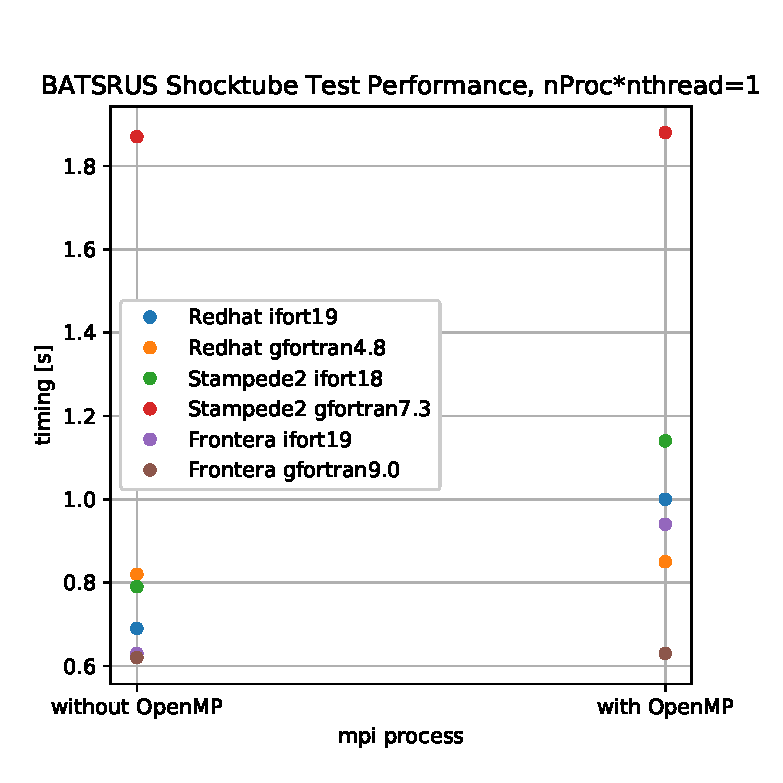
\includegraphics[width=\textwidth]{./figures/shocktube_timing_1}
    \caption{Comparisons of BATSRUS compiling with or without OpenMP flag.}
    \label{fig:shocktube_timing1}
\end{figure}

\begin{figure}[h]
    \centering
    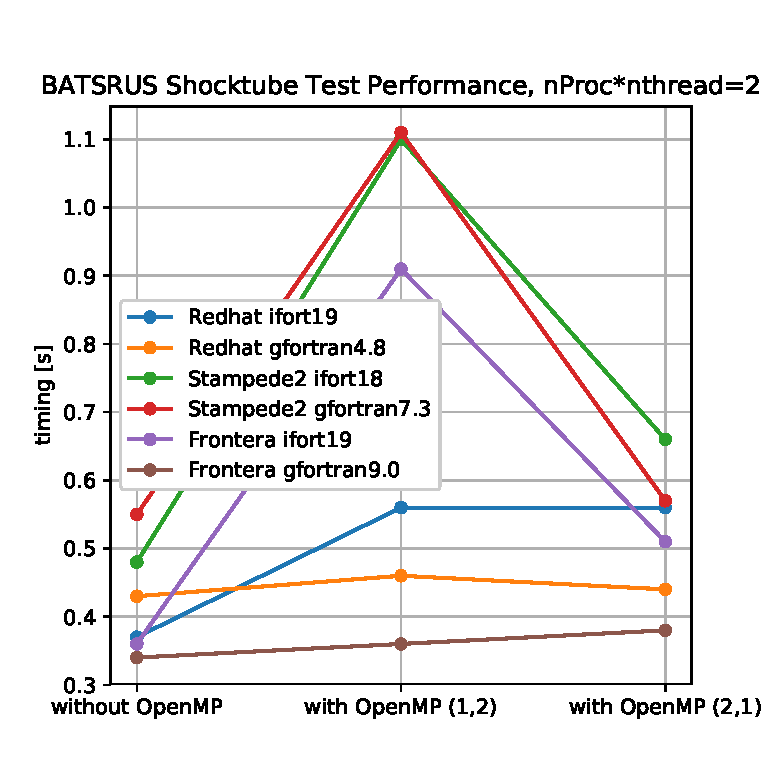
\includegraphics[width=\textwidth]{./figures/shocktube_timing_2}
    \caption{Comparisons of BATSRUS compiling with or without OpenMP flag. Three vertical lines represent 2 MPI compiling without OpenMP, 1 MPI and 2 threads, and 2 MPI and 1 thread.}
    \label{fig:shocktube_timing2}
\end{figure}

\begin{figure}[h]
    \centering
    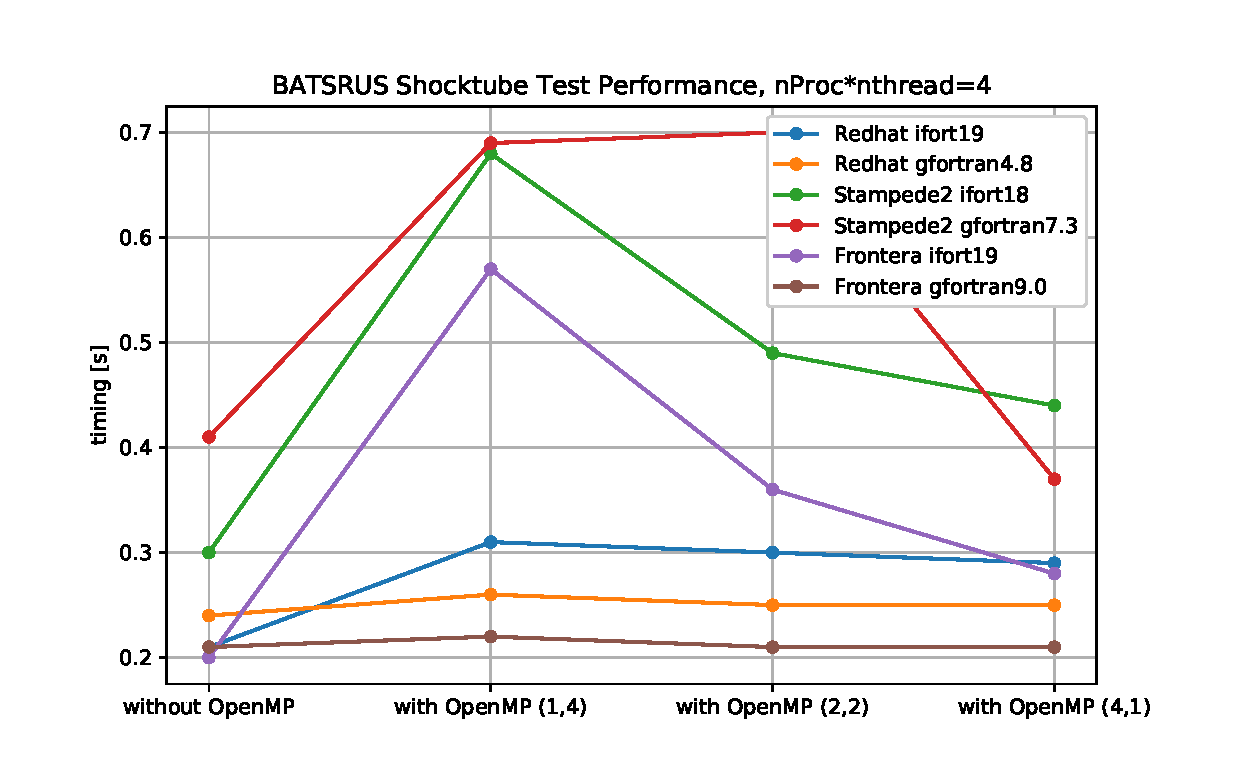
\includegraphics[width=\textwidth]{./figures/shocktube_timing_4}
    \caption{Comparisons of BATSRUS compiling with or without OpenMP flag. Four vertical lines represent 4 MPI compiling without OpenMP, 1 MPI and 4 threads, 2 MPI and 2 threads, and 4 MPI and 1 thread.}
    \label{fig:shocktube_timing4}
\end{figure}

\verb|unused_B| is causing some performance issues.

Limiters in \verb|ModFaceValue.f90| may be improved. I tried, and failed. In flux limiters, intel detects anti-dependencies, but it left them unvectorized for $-O2$. Proven dependency? There also seems to be a lot of mispredicting branches.

Compiler suggests re-ordering the case and if statements.

\verb|get_physical_flux|: vectorize serialized functions inside loop

\textbf{Data alignment}

data not aligned: (because nVar is not a multipler of 4?)
\begin{verbatim}
primitive_VG = State_VGB(:,:,:,:,iBlock)
State_Old(:,:,:,:,iBlock) = State_VGB(:,:,:,:,iBlock)
\end{verbatim}

\begin{verbatim}
Flux_V = Flux_V * Area
\end{verbatim}
Ineffective peeled/remainder loop present

If anti-dependency exists, use a directive where k is smaller than the distance between dependent items in anti-dependency.

\verb|MPI_reduce| gets stuck with many MPI processes?

\textbf{Performance}

Compared the 2019/05/20 version with 2019/01/01, the current face flux calculation runs $\sim30\%$ slower in the Ganymede test!

Now I am trying the find out what causes the issue. The 2019/02/06 code seems closer to the 01/01 code performance.

My first guess is that Igor's MhdFlux or HdFlux has penalties. However, after some check this is not the case. In the end, surprisingly, the \verb|norm2| introduced in \verb|ModUtility| for pgfortran not implementing the intrinsic function is the reason! This causes $30\%$ performance loss with gfortran on Mac and $10\%$ loss with ifort on Linux for the flux calculation.

\textbf{Memory Deallocation}

Because BATSRUS is designed for multi-sessions, memories may be freed in the middle of the runs between sessions. There are potentially a lot of places where this is neglected.

\textbf{BATL API}

The BATL library now has a strange logic: there are multiple modules containing their own variables and functions, but they should be collected together so that a outside user can call them with a unique module name \verb|BATL_lib|. There are restrictions on this for some versions of ifort.

\textbf{Resistivity}

Why is \verb|set_resistivity| being called inside \verb|calc_heat_exchange|? It is actually called three times in one timestep for a second order scheme!

Calculate heat exchange tries to close the gap between ion and electron temperatures. Resistivity may change between runs, so it is reset every time. This may cause unnecessary work!

Additionally, a temperory array is allocated repeatedly, which is probably a waste of time.

\textbf{Another potential issue: Unused\_B(iBlock)}

If we use AMR, we may have unused blocks in the array. This means that the load balancing among threads may not be optimal. Depends how threads are launched. Maybe it works just fine. Could be interesting to test.

\textbf{OpenMP overhead}

I want to check if the openMP overhead by compiling with openMP is a fixed number or is dependent on the problem size.

%-----------------------------
\section{Code Structure}

On the highest level, there's a session loop which looks like

\smartdiagram[flow diagram]{
  setup,
  init\_session,
  advance,
  save,
  finalize}



\verb|ModMultiIon|: calculate source terms for multi-ion MHD, usually used with point-implicit schemes.

\verb|ModCalcSource|: module for calculating explicit/implicit source terms. Only one public function \verb|calc_source|

\verb|ModThreadedLC|: seems to be related to the sun. UseFieldLineThreads

\verb|Mod_Block_Data|: moves cache data from block to block for the sake of load balance and adaptive mesh refinement.


%-----------------------------
\section{OpenMP Modules}
Modules that are currently modified with OpenMP directives are:
\begin{itemize}
\item \verb|ModAdvance|
\item \verb|ModAdvanceExplicit|
\item \verb|ModB0|
\item \verb|ModBorisCorrection|
\item \verb|ModFaceFlux|
\item \verb|ModFaceGradient|
\item \verb|ModFaceValue|
\item \verb|ModFaceBoundary|
\item \verb|ModCellBoundary|
\item \verb|ModMultiFluid|
\item \verb|ModMultiIon|
\item \verb|ModPointImplicit|
\item \verb|ModViscosity|
\item \verb|ModCurrent|
\item \verb|ModFaceGradient|
\item \verb|ModWaves|
\item \verb|ModHallResist|
\item \verb|ModHeatConduction|
\item \verb|ModCoronalHeating|
\item \verb|ModRadDiffusion|
\item \verb|ModRadiativeCooling|
\item \verb|ModChromosphere|
\item \verb|ModUpdateState|
\item \verb|ModThreadedLC|
\item \verb|ModSemiImplicit|
\item \verb|ModResistivity|
\item \verb|ModPhysics|
\item \verb|ModPartImplicit|
\item \verb|ModMessagePass|
\item \verb|ModGeometry|
\item \verb|ModChromosphere|
\item \verb|BATL_region|
\item \verb|ModLinearSolver|
\item \verb|ModExactRS|
\item \verb|ModPhysics|
\item \verb|ModRestartFile|

\end{itemize}

Now \verb|exchange_energy|, \verb|update_check| are also multi-threaded. \verb|exchange_energy| is for transforming between temperature and energy?

\verb|ModConserveFlux| can be multi-threaded, but it is not currently because it takes too little time.

\verb|ModConstrain| is rarely used, so it is not multi-threaded.


%---------------------------------
\section{Multi-thread Tests}

Currently all the overnight tests for BAT-S-RUS are running with 2 threads. Table \ref{tab:night_test} summarizes the accuracy results.

\begin{table}[htbp]
  \centering
  \caption{BATSRUS nightly tests}
    \begin{tabular}{lcc}
    \toprule
    Test Name & Status & Description \\
    \midrule
    test\_func &   \\
    test18     & ? & $P_{max}$ diff \\
    test20     & ?   \\
    \midrule
    2bodyplot & \checkmark \\
    amr           & ? & time accurate, AMR, error down to machine $\epsilon$ \\
    anisotropic & \checkmark   \\
    awsomfluids  & \text{\sffamily X} & lack of input data files \\
    chromo  & \checkmark  & semi-implicit \\ 
    comet & \checkmark & point-implicit \\
    cometCGfluids & \checkmark & point implicit, BlockData \\
    cometCGhd & \checkmark  \\
    cometfluids & \text{\sffamily X} & point-implicit, crashed in \verb|ModUser| neutral atmosphere \\    
    cometfluids\_restart & \text{\sffamily X} &  \\
    corona & \checkmark \\
    coronasph & \checkmark & AMR \\
    earthsph & \checkmark &  part-implicit, difference in time-accurate run \\
    eosgodunov & \text{\sffamily X} & crash, cannot even run serial \\
    fivemoment\_alfven &\checkmark & explicit \\
    fivemoment\_langmuir & \checkmark & explicit \\
    fivemoment\_shock & \checkmark & point-implicit \\
    fluxemergence & \text{\sffamily X} & lack of include file \\
    ganymede & \checkmark & semi-implicit, at least works with serial implicit solver  \\
    graydiffusion & ? & full-implicit, hd, diff since 2 step\\
    hallmhd & \checkmark & semi-implicit, part-implicit, \verb|BATL_region| allocation\\
    laserpackage & \text{\sffamily X}\\
    magnetometer & \checkmark\\
    mars & \checkmark & fixed \verb|user_calc_sources| \\
    mars\_restart & \checkmark & fixed \verb|user_calc_sources| \\
    marsfluids & \checkmark & point-implicit \\
    marsfluids\_restart & \checkmark  \\
    mercurysph & \checkmark & explicit, Hall resistivity, \verb|BATL_region| \\
    mhdions & \checkmark &  point-implicit \\
    mhdnoncons & \checkmark \\
    multifluid & \checkmark \\
    multiion &\checkmark & point-implicit \\
    outerhelio & \checkmark &  \\
    outerheliopui & \checkmark &  fixed \verb|ModUser| \\
    partsteady & \checkmark & randomly crashed, sometimes good?\\
    region2d & \checkmark &  \\
    saturn & \checkmark & user sources \\
    shockramp & ? & $5^{th}$ order scheme, AMR, sometimes diff \\
    shocktube & \checkmark \\
    spectrum &\text{\sffamily X} & compile needs data \\
    titan &\checkmark & \verb|ModUser| similar to Mars \\
    titan\_restart &\checkmark \\
    twofluidmhd & \checkmark & \verb|ModUserWaves| \\
    venus & \checkmark & \verb|ModUser| similar to Mars  \\
    venus\_restart & \checkmark  \\
    viscosity & \checkmark & \verb|ModViscosity|, \verb|ModFaceFlux| \\
    \bottomrule
    \end{tabular}
  \label{tab:night_test}
\end{table}

\clearpage

\subsection{Auto-checker}

We had an idea of writing a script for automatically checking the module variables that are changing inside block loops. It is really interesting. Start from \verb|share/Scripts/AddTest.pl| for the regular expressions.

Always not sure about \verb|var_I| type of variables.


\subsection{Issues}

It is annoying that OpenMP doesn't have a threadprivate region syntax. I added the threadprivate declarations right after the variables.

\verb|user_calc_sources| in ModUserMars calls \verb|user_impl_source|, which is why multi-threading not working.

\verb|var_I| that is set at the initial time shouldn't be declared as threadprivate!

\begin{verbatim}
  !hyzhou: iBoundary,iFace,jFace,kFace is defined here only because they are                                          
  !used inside user_set_face_boundary. It would be much better if we could                                            
  !remove this prone-to-error usage!!!  
\end{verbatim}

It turns out that some var with \_I shouldn't be declared as threadprivate. Those that are set at the inital setup and used later should not be threadprivate.

\href{https://www.openmp.org/wp-content/uploads/finterp10.html#interp5}{openmp module var question}

\href{https://www.openmp.org/wp-content/uploads/finterp10.html}{An old openmp fortran question list}

I can see upper/lowercase difference in log file for Titan test.

Inside GMRES, there is a dot product for normalization. There doesn't seem to be a gain in speed if I use OpenMP workshare.

I fixed the problem that fully implicit solver cannot work in \verb|impl_newton_init| by adding threadprivate clause to \verb|ModHallResist| and \verb|ModWaves|.

For Mecury test,  it turns out that I missed the module variable \verb|Area| in \verb|BATL_region| and \verb|UseHallGradPe|.

Finally, this earthsph test passed! The final problem is in the rotation of the magnetic axis: \verb|omega_D| should be declared as threadprivate.

\textbf{Point implicit scheme debugging}

\verb|update_point_implicit| is called per thread.
\verb|update_state_normal|, if \verb|UsePointImplicit|, call \verb|update_point_implicit|
\verb|iVarPointImpl_I| shouldn't be threadprivate?

I now understand why the point-implicit solver shows some strange behaviours. That is all due to initializations?

I realized one big issue when passing function as an argument: OpenMP seems to totally ignore the function after the first evaluation? This \verb|user_calc_sources| is passed as a pointer to \verb|calc_point_impl_source|, and it is lost after one call!

Problem solved: that was due to the improper scope of some initialized logical variables in the function.
These logicals are set to true at the beginning of a loop and set back to false at the end of the loop. All those strange multi-thread behaviors show up if I don't declare them as \emph{threadprivate}: they are shared, they may change value in the middle of the loop due to the asynchronization execution of threads!

Now after a while, the issue showed up again, in cometfluids and europa2fluidsPe tests.

\textbf{Thread scheduling}

Load imbalance

\textbf{Nowait clause}


%-------------------------------------
\section{Point Implicit Scheme}
\begin{itemize}
\item \verb|read_point_impl_param|
\item \verb|init_point_implicit_num|
\item \verb|init_mod_point_impl|
\item \verb|clean_mod_point_impl|
\item \verb|update_point_impl|
\end{itemize}

In subroutine \verb|update_point_implicit(iBlock, calc_point_impl_source, init_point_implicit)|, the latter two arguments are functions.

\begin{lstlisting}[language=Fortran, caption=Point implicit scheme]
! Switch to implicit user sources
IspointImplSource = .true.

! Initialization

! Store explicit update
StateExpl_VC = State_VGB(:,1:nI,1:nJ,1:nK,iBlock)

! Put back old values into the implicit variables so the update is relative to time level n
State_VGB(iVar,i,j,k,iBlock) = StateOld_VGB(iVar,i,j,k,iBlock)

! Calculate unperturbed source for RHS
call calc_point_impl_source(iBlock)

! Calculate (part of) Jacobian numerically if necessary
if(.not.IsPointImplMatrixSet)then
   ...
end

! Do the implicit update
do k=1,nK; do j=1,nJ; do i=1,nI
   ! Do not update body cells
   if(.not.true_cell(i,j,k,iBlock)) CYCLE
   
   DtCell = Cfl*time_BLK(i,j,k,iBlock) * iStage / real(nStage)
   
   ! RHS is Uexpl - Uold + Sold
   do iIVar=1,nVarPointImpl
      iVar=iVarPointImpl_I(iIVar)
      Rhs_I(iIVar) = StateExpl_VC - StateOld_VGB + DtCell * Source_VC
   end
   
   ! The matrix to be solved for is A = (I - beta*Dt*dS/dU)
   do iIVar = 1, nVarPointImpl
      iVar = iVarPointImpl_I(iIVar)
      do iJVar = 1, nVarPointImpl
          jVar = iVarPointImpl_I(iJVar)
          Matrix_II(iIVar,iJVar) = - BetaStage*DtCell*DsDu_VVC(iVar,jVar,i,j,k)
       end do
       ! Add unit matrix
       Matrix_II(iIVar,iIVar) += 1,0
   end
   
   ! Solve A.dU = RHS
   call linear_equation_solver(nVarPointImpl,Matrix_II,Rhs_I)
   
   ! Update: U^n+1 = U^n + dU
   do iIVar=1,nVarPointImpl
      iVar = iVarPointImpl_I(iIVar)
      State_VGB(iVar,i,j,k,iBlock) = StateOld_VGB(iVar,i,j,k,iBlock) + Rhs_I(iIVar)
   end
  
   ! Set minimum density (no negative density allowed)
end; end; end

\end{lstlisting}

Point implicit solver is operated per block, so only a linear solver per block is required.


%-------------------------------------
\section{Part Implicit Scheme}
Part implicit means that only a portion of blocks are updated with implicit schemes. Obviously full implicit scheme is a subset of part implicit scheme. The main module consists of four functions:
\begin{itemize}
\item \verb|read_part_impl_param|
\item \verb|init_mod_part_impl|
\item \verb|clean_mod_part_impl|
\item \verb|advance_part_impl|
\end{itemize}

By default the Newton iteration is only performed one step. \verb|solve_linear_multiblock| chooses an implicit solver for all the implicit-treated blocks on the current processor.
The key part of algorithm:
\begin{lstlisting}[language=Fortran, caption=Part implicit scheme]
! Initialize some variables in ModImplicit
call implicit_init
! Get initial iterate from current state
call explicit2implicit

call MPI_allreduce(nImpl, nImplTotal)

call MPI_allreduce(NormLocal_V, Norm_V)

! Advance explicitly treated blocks if any
if(UsePartImplicit .and. nBlockExplALL > 0) then
   if(UseBDF2) then
      ! Save the current state into the previous state
      do iBlock=1,nBlock
         ...
      end
   end
   
   if(.not.UsePartImplicit2) then
      ! Select Unused_B = not explicit blocks
   end
   
   ! Advance explicit blocks
   call advance_explicit(.true., -1)
   
   if(.not.UsePartImplicit2) then
      ! update ghost cells for the implicit blocks to time level n+1
   end
   
   call exchange_messages
   
   ! Make sure the implicit scheme is only applied on implicit blocks 
end

!\
! Advance implicitly treated blocks
!/

! Let other parts of the code know that we are inside the implicit update 
! Switch off point implicit scheme (no need)
! Switch off merging the cells around the poles
! Use implicit time step

if(.not.UseBDF2)then
   ! Save the current state into ImplOld_VCB so that StateOld_VGB can be restored
end

! Initialize right hand side and x_I. Uses ImplOld_VCB for BDF2 scheme.     
call impl_newton_init

! Save previous timestep for 3 level scheme
if(UseBDF2)then
   !hyzhou: this is almost the same as not using BDF2!!!
end

! Newton-Raphson iteration and iterative linear solver
NormX = BigDouble
nIterNewton = 0
do
   nIterNewton = nIterNewton + 1
   if(nIterNewton > MxIterNewton)then
      error
      EXIT
   end if

   ! Calculate Jacobian matrix if required
   if(ImplParam%DoPrecond)then

   end

   ! Update rhs and initial x_I if required
   if(nIterNewton > 1) call impl_newton_loop

   ! Solve implicit system
   ! For Newton solver the outer loop has to converge,                      
   ! the inner loop only needs to reduce the error somewhat.

   if(UseNewton) ImplParam%ErrorMax = 0.1
   call solve_linear_multiblock

   if(ImplParam%iError /= 0) error; end

   ! Update w
   call impl_newton_update

   if(IsConverged) EXIT
end do 

if(UseConservativeImplicit) call impl_newton_conserve

! Put back implicit result into the explicit code
call implicit2explicit(Impl_VGB)

! Make explicit part available again for partially explicit scheme
if(UsePartImplicit)then
   ...
end

! Exchange messages, so ghost cells of all blocks are updated
call exchange_messages

\end{lstlisting}

%--------------------------------------
\section{Semi-implicit Scheme}
Semi-implicit scheme means that only part of the variables are solved with implicit schemes. The main module also consists of four functions:
\begin{itemize}
\item \verb|read_semi_impl_param|
\item \verb|init_mod_semi_impl|
\item \verb|clean_mod_semi_impl|
\item \verb|advance_semi_impl|
\end{itemize}

The key algorithm in \verb|advance_semi_impl|: 
\begin{lstlisting}[language=Fortran, caption=Semi-implicit scheme]
! Check semi-implicit blocks, store B field in SemiAll_VCB
call get_impl_resistivity_state(SemiAll_VCB)

do iVarSemi=1,nBarSemiAll,nVarSemi
   ! Set right hand side
   call get_semi_impl_rhs(SemiAll_VCB, Rhs_I)
   ! Calculate Jacobian matrix if required
   if(SemiParam%DoPrecond)then
      call get_semi_impl_jacobian
   end
   
   ! solve implicit system
   call solve_linear_multiblock
   
   if(SemiParam%iError /= 0) call error_report
   
   ! Update solution
   n = 0
   do iBlockSemi=1,nBlockSemi; do k=1,nK; do j=1,nJ; do i=1,nI
      do iVar=iVarSemiMin, iVarSemiMax
         n = n + 1
         if(true_cell)then
            ! update
         else
            ! no update
         end
      end
   end; end; end; end
end
   
! Put back semi-implicit result into explicit code
do iBlockSemi=1,nBlockSemi
   call update_impl_resistivity(iBlock, NewSemiAll_VCB(:,:,:,:,iBlockSemi))
end
\end{lstlisting}

\verb|get_semi_impl_rhs_block| is a wrapper which calls \verb|get_resistivity_rhs| in \verb|ModResistivity|.

Observation:
\begin{enumerate}
\item Key variables:
\subitem \verb|Rhs_I(nVarSemi*nIJK*MaxBlock)|
\subitem \verb|x_I(nVarSemi*nIJK*MaxBlock)|
\item Key functions:
\subitem \verb|solve_linear_multiblock|
\end{enumerate}

\begin{table}[htbp]
  \centering
  \caption{Implicit inputs}s
 \begin{tabular}{lll}
    \toprule
Variables                & Meaning           & Notes\\
\midrule         
\verb|SemiParam| & solver parameters  & derived type \\
\verb|nVarSemi|    & \# of implicit vars    & \verb|ModImplicit| \\
\verb|nDim,nI,nJ,nK,nBlockSemi| & grid info   & \verb|BATL_lib| \\
\verb|iComm| & communicator & \verb|ModProcMH|  \\
\verb|semi_impl_matvec| & Calculate $Rhs = Ax$  & function \\
\verb|Rhs_I| &  & nVarSemi*nIJK*MaxBlock\\
\verb|x_I| & & nVarSemi*nIJK*MaxBlock\\
\verb|DoTestKrylov| & & \\
\verb|JacSemi_VVCIB| &  Jacobian/preconditioner & nVarSemi,nVarSemi,nI,nJ,nK,nStencil,MaxBlock\\
\verb|JacobiPrec_I| & pointwise Jacobi preconditioner &  nVarSemi*nIJK*MaxBlock\\
\verb|cg_precond| & CG preconditioner & function\\
\verb|hypre_preconditioner| & & ModImplHypre \\
    \bottomrule
    \end{tabular}
  \label{tab:impl_input}
\end{table}

\verb|Rhs_I| is calculated by \verb|semi_impl_matvec|, which is actually calculated in \verb|solve_linear_multiblock|. This is called inside, for example, the Krylov loop. For the MPI version, each processor calls this solver once per time step.

\verb|semi_impl_matvec| is the key part:
\begin{lstlisting}[language=Fortran, caption=Semi-implicit matvec]
! Fill in SemiState so it can be message passed
SemiState_VGB = SemiAll_VCB

! Message pass to fill in ghost cells
call message_pass_cell(nVarSemi, SemiState_VGB)

do iBlockSemi=1,nBlockSemi
   ! Apply boundary conditions (1 layer of outer ghost cells)
   if(far_field_BCs_BLK(iBlock)) call set_cell_boundary
   
   call get_semi_impl_rhs_block
end

! Multiply with cell volume ( makes matrix symmetric)
do iBlockSemi=1,nBlockSemi
   RhsSemi_VCB *= CellVolume_GB
end

if(UseStableImplicit)then
   ...
end
\end{lstlisting}


\verb|get_semi_impl_rhs_block|: wrapper for radiation/heat conduction/resistivity calls.

\verb|get_resistivity_rhs|: get \verb|Rhs_VC| from \verb|StateImpl_VG| for each block

\begin{lstlisting}[language=Fortran, caption=???]
do iBlockSemi=1,nBlockSemi
   SemiState_VGB = SemiAll_VCB
end do

call message_pass_cell(SemiState_VGB)

do iBlockSemi=1,nBlockSemi
   call get_semi_impl_rhs_block(iBlock, SemiState_VGB, RhsSemi_VCB)
end do

do iBlockSemi=1,nBlockSemi
   Rhs_I =  f(ResSemi_VCB)
end do
\end{lstlisting}

\dirtree{%
.1 advance\_semi\_impl.
.2 get\_semi\_impl\_rhs.
.3 message\_pass\_cell.
.3 set\_cell\_boundary.
.3 get\_semi\_impl\_rhs\_block.
.3 message\_pass\_face.
.3 apply\_flux\_correction\_block.
.2 solve\_linear\_multiblock.
.3 semi\_impl\_matvec.
.4 message\_pass\_cell.
.4 set\_cell\_boundary.
.4 get\_semi\_impl\_rhs\_block.
.5 get\_rad\_diffusion\_rhs.
.5 get\_heat\_conduction\_rhs.
.5 get\_resistivity\_rhs.
.4 message\_pass\_face.
.4 apply\_flux\_correction\_block.
.4 semi\_precond.
.2 update\_impl\_*.
}


\subsection{Solution}

There are four parts of the implicit solver that can be multi-threaded:
\begin{enumerate}
\item wrap the state variables into 1D long arrays and unwrap them after the iterative solver;
\item building the preconditioner;
\item \verb|matvec|
\item \verb|matmul(x_I,y_I)| inside the implicit Krylov solver.
\end{enumerate}

By testing, I found that calling function \verb|matvec| dominates the time on one processor. The timing report shows that matrix multiplication takes about 30\% of the total execution time.


%----------------------
\section{Testing}

\subsection{Strong scaling}



test case
compiler, optimization


Grid (cell + block)

mpi + openmp

The results for the implicit scheme are not very steady. 2 thread cases gives completely different timings!

\begin{figure}[h]
    \centering
    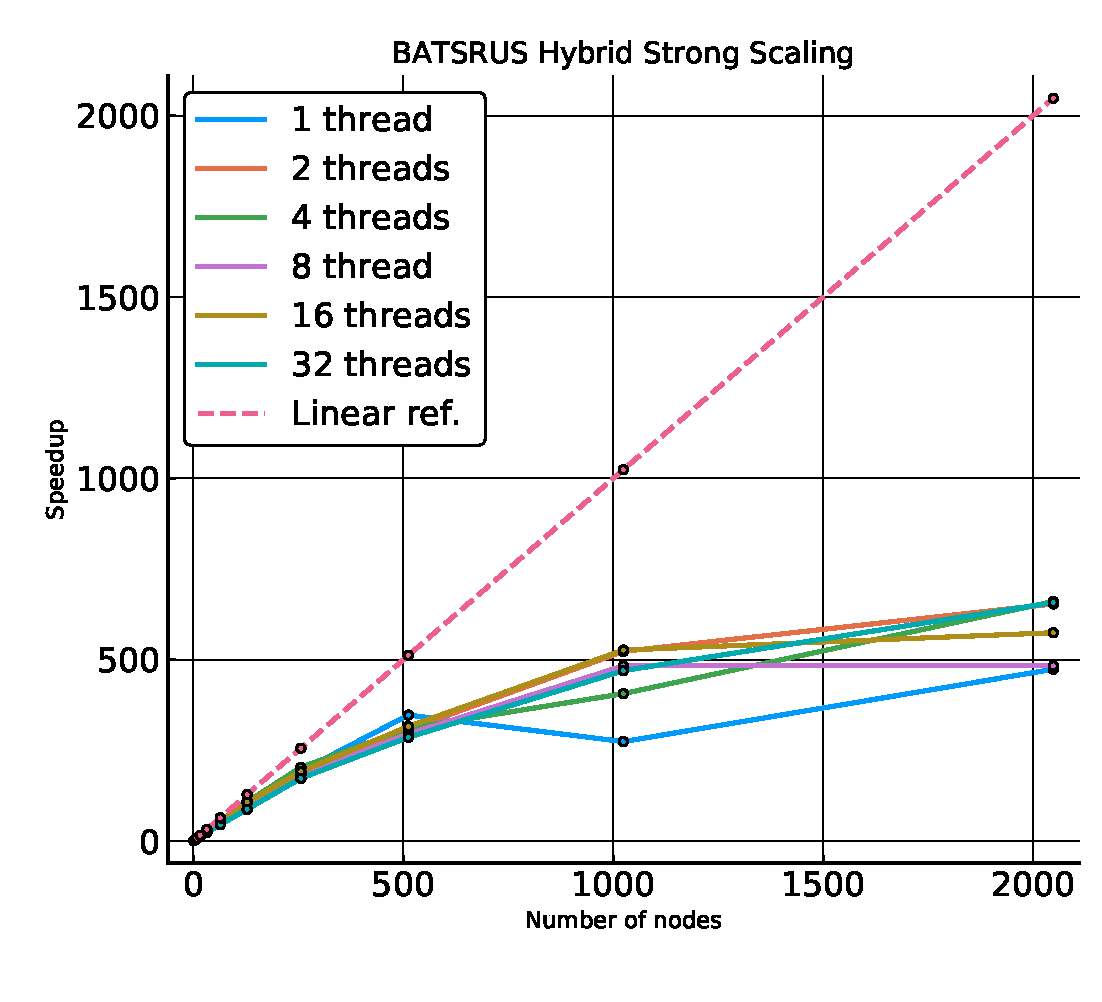
\includegraphics[width=\textwidth]{./figures/StrongScale_base32_linear}
    \caption{BAT-S-RUS hybrid strong scaling tests of 3D shocktube problem using second order explicit Linde scheme on Bluewaters. Each computing node has two AMD 6276 Interlagos processors, and a single XE node has 32 ``integer'' cores. The number of blocks per core ranges from 2048 to 1 for single thread runs.}
    \label{fig:StrongScale}
\end{figure}


\subsection{Weak scaling}

% I will add another zoom in figure at the bottom right part!
\begin{figure}[h]
    \centering
    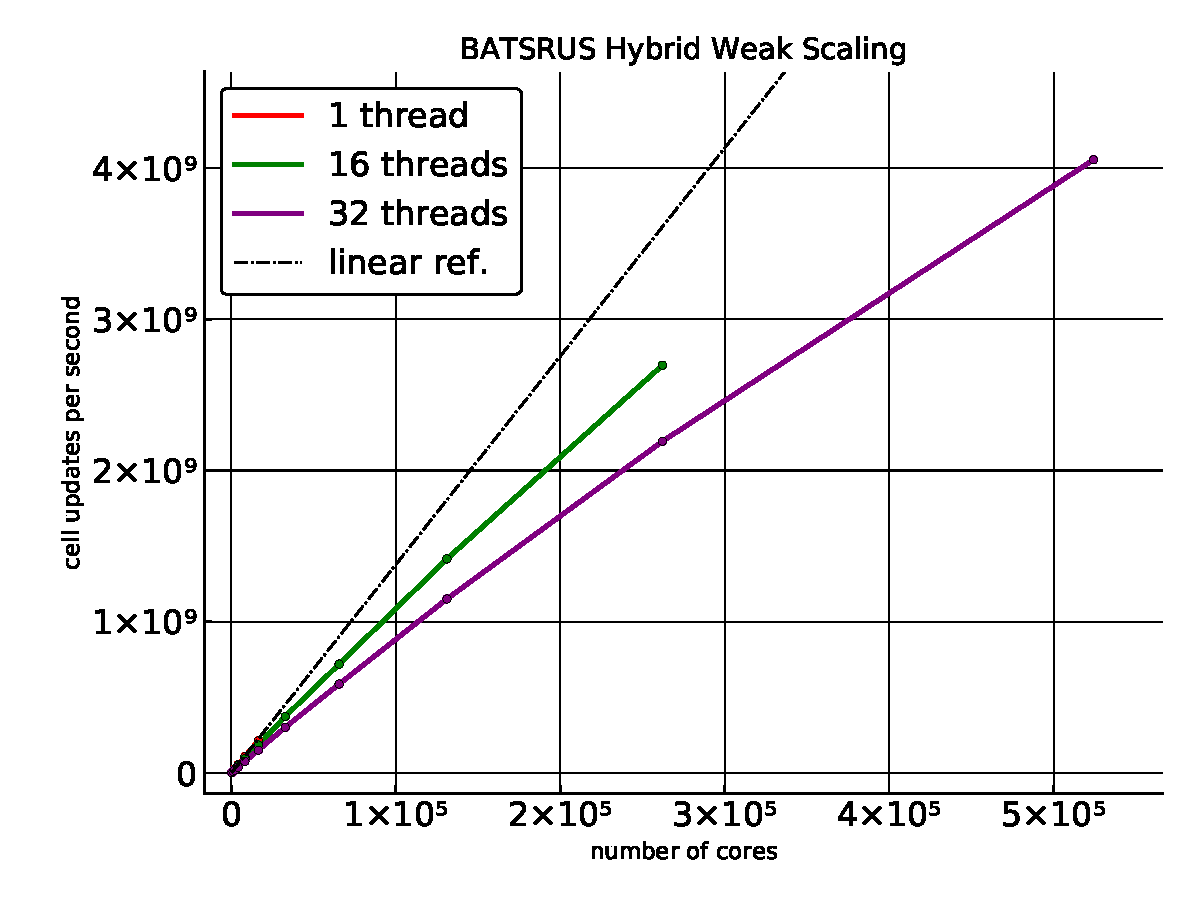
\includegraphics[width=\textwidth]{./figures/WeakScale_linear}
    \caption{BAT-S-RUS hybrid weak scaling tests of 3D shocktube problem using second order explicit Roe scheme on Bluewaters. Each computing node has two AMD 6276 Interlagos processors, and a single XE node has 32 ``integer'' cores. The number of blocks per core ranges from 2048 to 1 for single thread runs.}
    \label{fig:WeakScale}
\end{figure}

%---------------------
\section{BATL}

My first attempt to modify \verb|BATL_pass_cell| failed. Although it can run successfully, but it takes more time than the original version, which is very sad to me. I compared the performance both with no optimization and with optimization, and the old version always beats my first version. For 1 MPI, sure it does speed up with multithreads; but with MPI calls for muliple MPIs, it slows down.

The problem for the first attempt turns out to be memory allocation of \verb|Slope_VG| every time in the block loop. The performance degraded because of this memory allocation.

Something is wrong with \verb|advect33_sph|. 

Here comes the third attempt. Accidentally, I found that doing local copy in another block loop after preparing the remote copy buffer gives significant improvement in terms of speed, especially for large thread numbers. This is probably due to the compiler optimization with a certain logical instead of running decision. Also for our cases, whether or not the location of local passes is after waitall or before waitall almost doesn't matter! Now it gives almost perfect timing all the way up to 8 threads; 16 is pretty good; 32 is ok. The best performance is achieved with 2 threads.

Why the pure MPI code fails at 32768 cores: the tree structure allocations in \verb|BATL_tree|:
\begin{enumerate}
\item \verb|iTree_IA|: $32768 [\text{cores}] * 256 [\text{blocks/core}]*18 [\text{integers/block}] * 4 [\text{byte}] *2\approx 1$GB
\item \verb|iNodeMorton_I|: $32768*256*2*4$
\item \verb|iMortonNode_A|: $32768*256*2*4$
\item \verb|iStatusNew_A|: $32768*256*2*4$
\item \verb|iStatusAll_A|: $32768*256*2*4$
\item \verb|iProcNew_A|: $32768*256*2*4$
\item \verb|iNodeNew_A|: $32768*256*2*4$
\end{enumerate}

The 2 for each array accounts for the possible adaptive mesh refinement.
All together these take about $2$GB of memory, which exceeds the memory limit per core on Bluewaters.

%---------------------
\section{Tecplot}

I want to the smooth the process of writng tecplot outputs. Right now we are saving finite element type data in ACSII format from each processor, using post-processing executables to merge the data and connectivities into one large ACSII file, and then using preplot to transform it into binaries. This is a practical bottleneck for doing real simulation work.

The open source TecIO library provides functions to read and write tecplot formats easily. It relies on the boost library in C++ and has an interface to Fortran. In the first stage, I successfully linked the library to BATSRUS and made some dummy outputs from each processor. Then I need to design the workflow for a better IO. Remaining questions are:
\begin{enumerate}
\item Can I write to the same output file in parallel with TecIOMPI?
\item If I choose to write output for each processor separately, how can I combine all the pieces into one large binary file?
\end{enumerate}

I am suffering from this right now. A nice solution to me now is to write one grid file (assuming no AMR) and one solution file per timestep. But I don't understand how szplt works! What are partitioned zones?

n TecIO, the portion of a zone on an MPI rank is called a partition. The use of partitions to write a single file from multiple processors is described in section 3-3 of the Tecplot 360 Data Format Guide. It only requires a couple more API calls to write the data in parallel. The most complicated part is dealing with overlapping, or ghost nodes, in the data. A couple of the example applications in the TecIO package write partitioned files. Check out brickpartitioned.cpp (or .F90)

%---------------------
\section{Future Development}

One thing to try for sure is OOP.

Using \verb|threadprivate| works, but this is not good for reading codes, maintainance and performance.
Readers cannot quickly catch the logic flow; maintainers are confused by the variables flying around functions; performance decreases because \verb|threadprivate| variables are allocated on heaps instead of stacks.

Quoted from the paper Techniques Supporting threadprivate in OpenMP:
\begin{verbatim}
threadprivate must be used with care. Do not consider that a threadprivate
variable can be as efficient as a private variable. Threadprivate implies that 
variables must be placed in common blocks to be kept save across parallel
regions. This may prevent some optimizations, like keeping values in registers
and the code will be slower. So use threadprivate only when the variables 
involved need to keep their values across functions and parallel regions.
\end{verbatim}

Implementation of \verb|threadprivate| based on thread-local storage (TLS) is implemented in linux gfortran compiler and greatly reduced the overhead.

In the long run, a far better approach may be to make the flows of information in your program explicit to a reader of the code (and more flexibly configurable by a code writer), by passing information as arguments (perhaps bundled together in derived types) rather than hiding those flows through the use of global (module) variables.

\subsection{Flux Calculation}

I have a plan for rewriting the whole flux module. Goals:
\begin{enumerate}
\item Eliminate the usage of module private variables.
\item Eliminate passing scalars between modules except constants.
\item Try to use submodules for different schemes?
\item Do I need to keep cell center flux calculations?
\item Figure out a way to separate the implicit solver with the face flux calculation, e.g. DoTestCell.
\end{enumerate}

\subsection{Point Implicit Scheme}

Try to eliminate the logicals for initiating the scheme!

\subsection{Test Module}

I don't like the current implementation of test functionalities, both the results checking and the subroutine tests.

%---------------------
\chapter{Parallel Affinity Control}

The matter of thread affinity becomes important on multi-socket nodes.

Thread placement can be controlled with two environment variables:
\begin{enumerate}
\item \verb|OMP_PROC_BIND|: describes how threads are bound to OpenMP places
\item \verb|OMP_PLACES|: describes these places in terms of the available hardware.
\end{enumerate}

When you're experimenting with these variables it is a good idea to set \verb|OMP_DISPLAY_ENV| to true, so that OpenMP will print out at runtime how it has interpreted your specification.

\section{Thread Binding}

The variable \verb|OMP_PLACES| defines a series of places to which the threads are assigned.

\underline{Example 1}: if you have two sockets and you define \verb|OMP_PLACES|=sockets, then it goes like round-robin.

\underline{Example 2}: if the two sockets have a total of sixteen cores and you define
\verb|OMP_PLACES|=cores ,\verb|OMP_PROC_BIND|=close, then it goes successively through the available places.

\underline{Example 3}: if the two sockets have a total of sixteen cores and you define
\verb|OMP_PLACES|=cores ,\verb|OMP_PROC_BIND|=spread, then it goes round-robin alternatively on the two sockets.

So you see that \verb|OMP_PLACES|=cores and \verb|OMP_PROC_BIND=spread| very similar to \verb|OMP_PLACES|=sockets . The difference is that the latter choice does not bind a thread to a specific core, so the operating system can move threads about, and it can put more than one thread on the same core, even if there is another core still unused.

The value \verb|OMP_PROC_BIND|=master puts the threads in the same place as the master of the team.

\section{Effects of Thread Binding}

Let's consider two example program. First we consider the program for computing $\pi$, which is purely compute-bound.

We see pretty much perfect speedup for the \verb|OMP_PLACES|=cores strategy; with \verb|OMP_PLACES|=sockets we probably get occasional collisions where two threads wind up on the same core.


%figure


Next we take a program for computing the time evolution of the heat equation:
\[
t=0,1,2,…:\forall_i : x_i^{t+1} = 2x_i^t - x_{i-1}^t - x_{i+1}^t
\]

This is a bandwidth-bound operation because the amount of computation per data item is low.


%figure

\section{Place Definition}

There are three predefined values for the \verb|OMP_PLACES| variable: \emph{sockets, cores, threads}. You have already seen the first two; the threads value becomes relevant on processors that have hardware threads. In that case, \verb|OMP_PLACES|=cores does not tie a thread to a specific hardware thread, leading again to possible collisions as in the above example. Setting \verb|OMP_PLACES|=threads ties each OpenMP thread to a specific hardware thread.

There is also a very general syntax for defining places that uses a
\begin{verbatim}
location:number:stride
\end{verbatim}
syntax.

\underline{Examples}:
\begin{enumerate}
\item \verb|OMP_PLACES|="\{0:8:1\},\{8:8:1\}" on a two-socket design

Equivalent to \emph{sockets} on a two-socket design with eight cores per socket: it defines two places, each having eight consecutive cores. The threads are then places alternating between the two places, but not further specified inside the place.
\item \verb|OMP_PLACES|="\{0\},\{1\},\{2\},...,\{15\}"

Equivalent to \emph{cores}.
\item \verb|OMP_PLACES|="\{0:4:8\}:4:1" on a four-socket design

states that the place 0,8,16,24 needs to be repeated four times, with a stride of one. In other words, thread 0 winds up on core 0 of some socket, the thread 1 winds up on core 1 of some socket, et cetera.
\end{enumerate}


\section{Binding Possibilities}

Values for \verb|OMP_PROC_BIND| are: \emph{false, true, master, close, spread}.
\begin{enumerate}
\item master: collocate threads with the master thread.
\item close: place threads close to the master in the places list.
\item spread: spread out threads as much as possible.
\end{enumerate}

A safe default setting is
\begin{verbatim}
export OMP_PROC_BIND=true
\end{verbatim}
which prevents the operating system from migrating a thread. This prevents many scaling problems.

As an example, consider a code where two threads write to a shared location.
\begin{lstlisting}[language=C, caption=sharing]
// sharing.c
#pragma omp parallel
  { // not a parallel for: just a bunch of reps
    for (int j = 0; j < reps; j++) {
#pragma omp for schedule(static,1)
      for (int i = 0; i < N; i++){
#pragma omp atomic
	a++;  
      }
      
    }
  }
\end{lstlisting}

There is now a big difference in runtime depending on how close the threads are. We test this on a processor with both cores and hyperthreads. First we bind the OpenMP threads to the cores:
\begin{verbatim}
OMP_NUM_THREADS=2 OMP_PLACES=cores OMP_PROC_BIND=close ./sharing
run time = 4752.231836usec
sum = 80000000.0
\end{verbatim}
Next we force the OpenMP threads to bind to hyperthreads inside one core:
\begin{verbatim}
OMP_PLACES=threads OMP_PROC_BIND=close ./sharing
run time = 941.970110usec
sum = 80000000.0
\end{verbatim}
Of course in this example the inner loop is pretty much meaningless and parallelism does not speed up anything:
\begin{verbatim}
OMP_NUM_THREADS=1 OMP_PLACES=cores OMP_PROC_BIND=close ./sharing
run time = 806.669950usec
sum = 80000000.0
\end{verbatim}
However, we see that the two-thread result is almost as fast, meaning that there is very little parallelization overhead.


\section{Affinity control outside OpenMP}

There are various utilities to control process and thread placement.

Process placement can be controlled on the Operating system level by \verb|numactl|. Each compiler has its own way to setting the thread affinities. Check them out for a specific machine.


%---------------------
\chapter{MHD Code Design}

\section{Principles}

\begin{itemize}
\item SOLID: Single Responsibility, Open/Closed, Liskov Substitution, Interface Segregation, Dependency Inversion
\item DRY: Don't Repeat Yourself
\item KISS: Keep It Simple, Stupid!
\item POLA: Principle of Least Astonishment
\item YAGNI: You Aren't Gonna Need It
\item POLP: Principle of Least Privilege
\end{itemize}

\section{}

Do not duplicate codes. For example, in the boundary condition setup, you should not write individual functions for different dimensions. This will lead to hard-to-follow codes as well as hard-to-detect bugs.

\section{References}

Enzo has cuda involved! It is in C. It probably uses 1D index for multi-dimensional arrays.

\href{http://enzo-project.org}{Enzo}

\href{https://bitbucket.org/enzo/enzo-dev}{Enzo source code}

Athena has the most complete description and code design in C++!

\href{https://princetonuniversity.github.io/athena/}{Athena}

Gamera

See the Matlab source code.

BATSRUS has now become a monster. I have an idea of rewrite the kernel structure to make it more like LEGO.

\section{Data Structure}

Almost all the C++ code has their own template for multi-dimensional arrays. From what I can see, each variable is stored continuously in the grid, instead of being stored altogether. I feel like this is faster than what we do in BATSRUS.

For example, in Enzo each variable is stored separately, but there is a Field Type ID defined for finding specific variable. In Athena (C++), a 4D array of size $[\text{N4}\times \text{N3}\times \text{N2}\times \text{N1}]$ is accessed as
\begin{verbatim}
A(n,k,j,i) = A[i + N1*(j + N2*(k + N3*n))]
\end{verbatim}
where the trailing index inside the parentheses is indexed fastest.

According to my test in my Matlab MHD code, this gives about $20\%$ speed up for the face flux calculation, and up to $10\%$ speed up for the source term calculation.

If I want to test with BATSRUS, I need to write a script to substitute all the patterns.

For a block-based code, there is always this question of where to put the global variables and ``local'' variables per block.
I don't like current solution in BATSRUS that messes everything together!

We can start from a clean version of BATSRUS, and gradually move all those threadprivate block-local variables inside functions. A nice solution would be, for example, create a class for storing all the block-independent intermediate variables. In this way we can avoid passing too many arguments among functions.

We need OOP features to write clearer codes!

\section{Numerical Schemes}

There are many numerical schemes to choose from. I really like Athena's idea of selecting a specific solver during compilation time instead of runtime: we can avoid many unnecessary complexities of branching inside loops and surely achieve better performance. If you think about it, who don't have time to compile the code if they need to switch to another scheme?

Likewise, the extra features like multi-fluid, multi-species and six-moments should all be separated.

Based on my test results, Gabor's \verb|ModFaceFlux| is very well written so that including 4 or 5 scheme together does not result in tramendous slow down. However, even if this reduces the total number of lines, it is really not good for maintainance. Any new comer to the code would find it hard to follow as so many branches are seen within several layers of function calls. It would be much cleaner to separate each scheme, just like the idea of object oriented programming.

For finite difference schemes, working on the grid is essentially equivalent to doing convolutions.

For the implicit solvers, find for the most suitable packages, instead of writing your own. For example, in Julia there is \verb|IterativeSolvers.jl| that is ready for usage. It both supports matrix and matrix-free form.

\section{Grid}

I want a block mesh generator with AMR. AMRex seems now to be the optimal choice besides BATL. Otherwise I should write my own mesh library in probably Julia.

AMRex currently has successful implementation in both PIC and fluid code. It is possible to combine the two approaches within the same framework. I should evaluate how complicated AMRex is before I actually start something.


\section{Timings}

\begin{table}[]
\begin{tabular}{llllll}
\hline
           & nCell & nWork & nBlock & nIter & time   \\
           \hline
CPU        & 8     & 10    & 1000   & 100   & 12.5   \\
GPU        & 8     & 10    & 1000   & 100   & 9.4    \\
CPU        & 8     & 100   & 100    & 1000  & 197.8  \\
GPU        & 8     & 100   & 100    & 1000  & 12.0   \\
CPU\_block & 8     & 100   & 100    & 1000  & 58.6    \\
GPU\_block & 8     & 100   & 100    & 1000  & 0.4    \\
CPU\_block & 8     & 1000  & 200    & 1000  & 1259.8 \\
GPU\_block & 8     & 1000  & 200    & 1000  & 1.6    \\
CPU        & 8     & 100   & 10     & 1000  & 19.8   \\
GPU        & 8     & 100   & 10     & 1000  & 1.3    \\
CPU        & 8     & 10    & 10000  & 10    & 12.7   \\
GPU        & 8     & 10    & 10000  & 10    & 9.5    \\
CPU        & 8     & 10    & 100    & 1000  & 12.4   \\
GPU        & 8     & 10    & 100    & 1000  & 9.5    \\
CPU        & 8     & 50    & 100    & 1000  & 88.6   \\
GPU        & 8     & 50    & 100    & 1000  & 10.4   \\
CPU        & 16    & 10000 & 1      & 1000  & 216.8  \\
GPU        & 16    & 10000 & 1      & 1000  & 2.6    \\
CPU        & 16    & 10000 & 1      & 100   & 21.7   \\
GPU        & 16    & 10000 & 1      & 100   & 0.4    \\
CPU        & 16    & 100   & 10     & 1000  & 149.4  \\
GPU        & 16    & 100   & 10     & 1000  & 1.4    \\
CPU        & 16    & 100   & 10     & 100   & 14.9   \\
GPU        & 16    & 100   & 10     & 100   & 0.3    \\
CPU        & 16    & 10    & 10     & 1000  & 9.1    \\
GPU        & 16    & 10    & 10     & 1000  & 1.2    \\
CPU        & 16    & 10    & 100    & 1000  & 91.4   \\
GPU        & 16    & 10    & 100    & 1000  & 10.5   \\
CPU        & 32    & 10    & 10     & 1000  & 70.0   \\
GPU        & 32    & 10    & 10     & 1000  & 2.0    \\
CPU        & 32    & 10    & 100    & 1000  &        \\
GPU        & 32    & 10    & 100    & 1000  & 22.0       \\
CPU        & 32    & 100   & 10     & 1000  & 1160   \\
GPU        & 32    & 100   & 10     & 1000  & 2.3    \\
CPU        & 32    & 100   & 1      & 1000  & 116.0  \\
GPU        & 32    & 100   & 1      & 1000  & 0.37   \\
CPU        & 64    & 100   & 10     & 100   & 913.3  \\
GPU        & 64    & 100   & 10     & 100   & 1.2   \\
\hline
\end{tabular}
\caption{Timings for the skeleton BATSRUS for porting to GPU with OpenACC}
\end{table}


\end{document}